\chapter{Multiscale Methods for polarized maps on the Sphere}
\label{ch_mms_pola}

% chapter multiscale transform for pola data

\section{Module-phase non linear multiscale transform}
%---------------------------------------------------------------------------------------------------------------------------------------
\label{sec:modphase}

\subsection{Introduction}
Given a polarized map in the standard Q-U representation, consider a different point of view and define the modulus $M$ and phase $P$ maps as follows~:
%
%From a different point of view, the combined $Q$ and $U$ maps can be considered as a vector field. Let define such combined map $\mathcal{V}$ as follows~:
%\begin{equation}
%{\mathcal{V}} = \left[ Q \, U\right]
%\end{equation}
%Each pixel of $\mathcal{V}$ is then vector valued. A classical approach amounts to decomposing each vector into its modulus and phase part. $\mathcal{V}$ can then be decomposed into a modulus map $M$ and a phase map $P$~:
\begin{eqnarray}
\forall k,\,\,\, M_k & = & \sqrt{Q_k^2 +  U_k^2} \\
\forall k,\,\,\, P_k & = & \exp(i \theta_k) \mbox{ where } tan(\theta_k) = U_k/Q_k 
\end{eqnarray}
Because the smoothness of the $Q$ and $U$ maps should result in some smoothness of the modulus map $M$ and the phase map $P$, 
one may consider devising a multiscale modulus/phase decomposition of the spin 2 field ${\mathcal{V}} = \left[ Q \, U\right]$.\\

The specificity of the modulus/phase decomposition of $\mathcal{V}$ is twofold~: i) the modulus field is non-negative and ii) the phase 
field takes its values on the unit circle $S^1$. Recently, \cite{rahman05} introduced a multiscale analysis technique for manifold valued 
data that will be described in the following paragraph. We then define the modulus/phase (MP) multiscale transform as follows~:
\vspace{.1cm}
\begin{center}
\begin{minipage}[b]{0.85\linewidth}
\footnotesize{
\begin{enumerate}
\item Apply a classical multiscale transform (\textit{i.e.} wavelets) to the modulus map $M$.
\item Apply the multiscale analysis technique for manifold valued data described in \cite{rahman05} to the phase map $P$. 
\end{enumerate}}
\end{minipage}
\end{center}
\vspace{.1cm}

\subsection{Decimated MP-multiscale transform}

\begin{figure*}[htb]
\centerline{
 \vbox{
 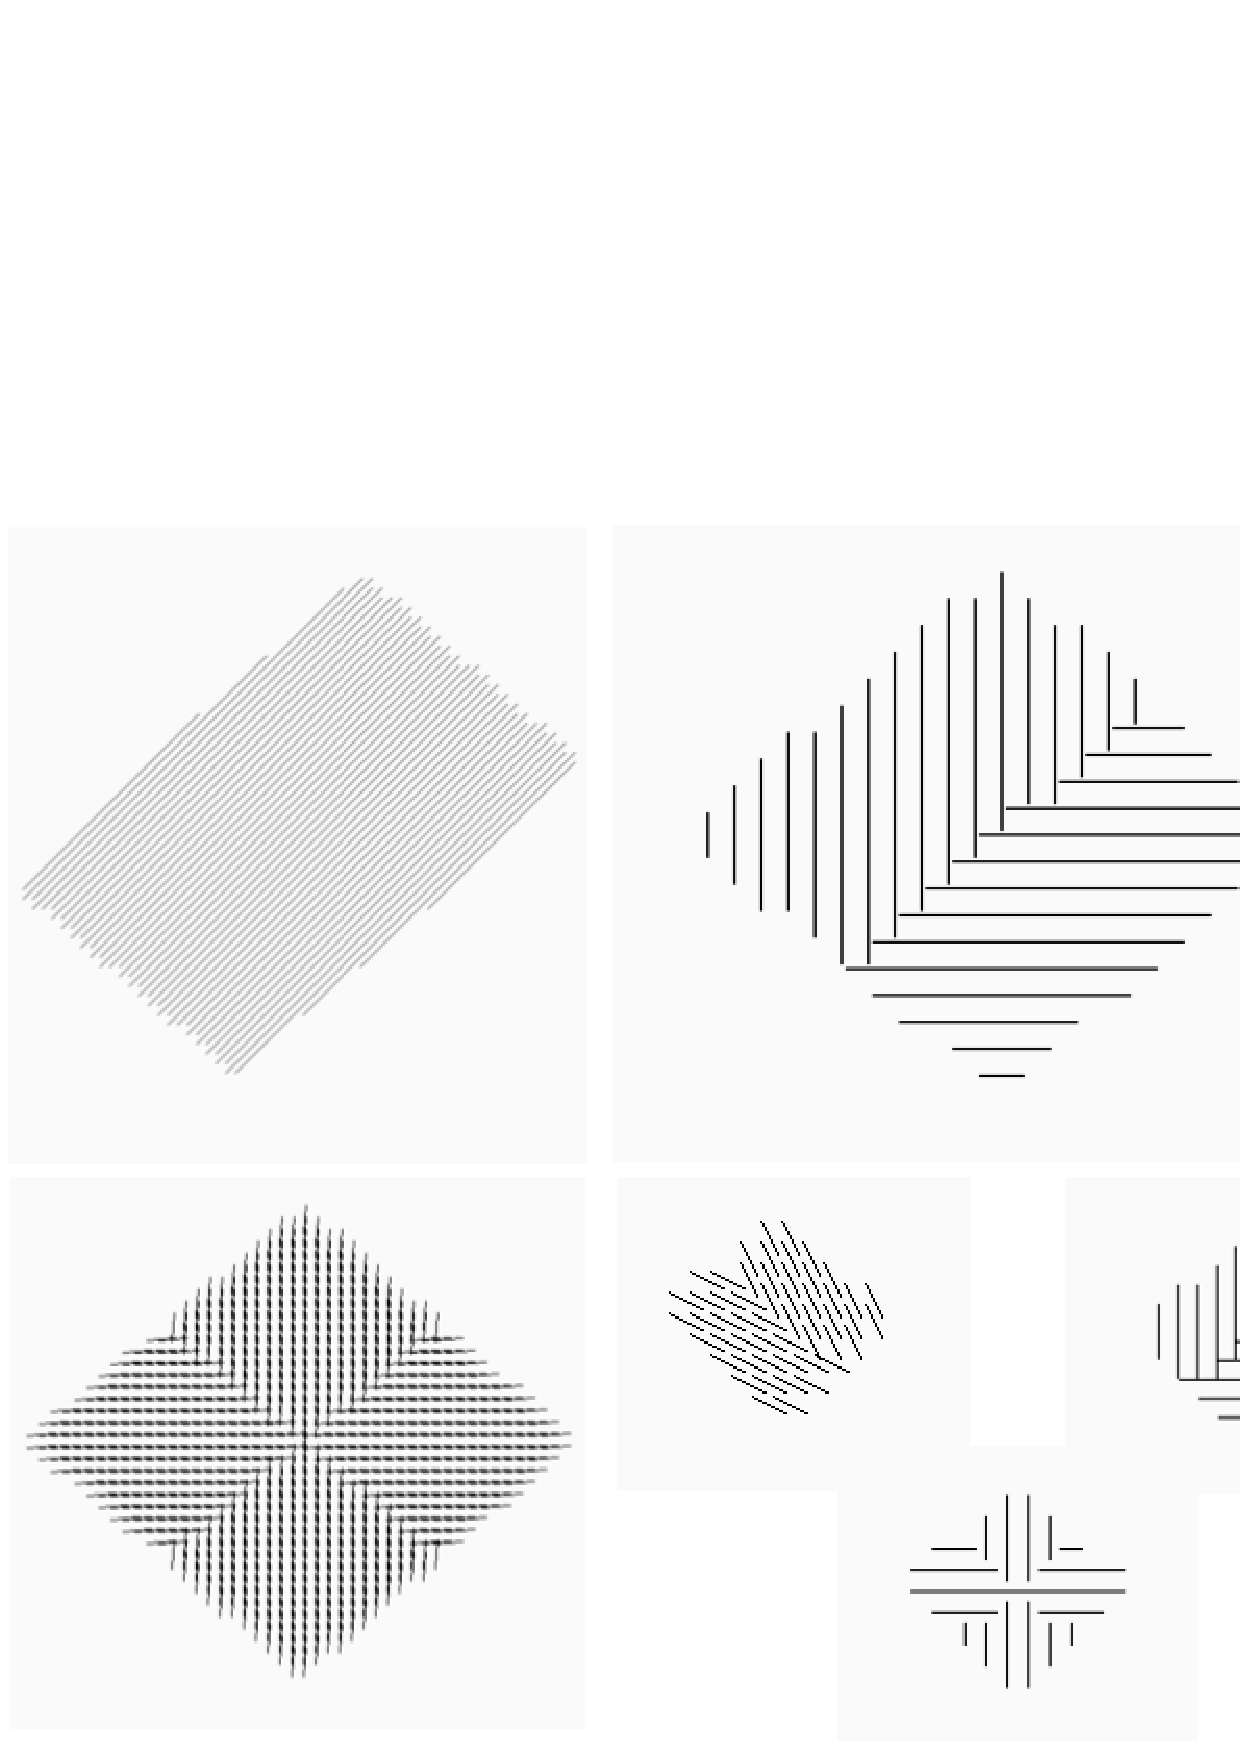
\includegraphics[width=\textwidth]{fig_modphase_back.pdf}
 }
 }
\caption{Examples of MP-multiscale coefficients backprojection.}
\label{fig_modphase_back}
\end{figure*}
Let us provide some essential notation~: we assume that the entries of the phase map $P$ lie in a manifold $\mathcal{M}$ 
(\textit{e.g.} $\mathcal{M}\equiv S^1$). According to \cite{rahman05}, take $p_0,p_1 \in \mathcal{M}$ and define $Log_{p_0}(p_1)$ 
as the log-map of $p_1$ onto the tangent space $\mathcal{T}_{p_0}$ of $\mathcal{M}$ at $p_0$. The back-projection is obtained 
using the inverse of the log-map $Exp_{p_0}$. \footnote{In differential geometry, the Exp map and Log map are generalizations of 
the usual exponential and logarithm function. Here the manifold $\mathcal{M}$ is a Riemannian manifold. In that case, the Exp map 
at point $p_0$, $Exp_{p_0}(s)$ is the map which takes a vector $s$ of the tangent space of $\mathcal{M}$ at $p_0$ and provides the 
point $p_1$ by travelling along the geodesic starting at $p_0$ in the direction s.}\\
For instance, if we choose $\mathcal{M} \equiv S^1$ then $p_0 = \exp(i \theta_0)$ and $p_1 = \exp(i \theta_1)$. The $Exp_{p_0}$ and 
$Log_{p_0}$ maps are then defined as follows~:
\begin{eqnarray}
\forall p_1 \in S^, \,\,\,  Log_{p_0} (p_1) & = & \theta_1 - \theta_0 \\
\forall s \in \mathbb{R} \,\,\, Exp_{p_0} (s) & = & exp(i(\theta_0 + s))
\end{eqnarray}
The multiscale transform for manifold valued data introduced in \cite{rahman05} is equivalent to a two-step interpolation-refinement 
scheme similar to the lifting scheme described in~\cite{wave:sweldens98}. The wavelet coefficients and low pass approximation pixels 
are then computed as follows at each scale $j$ and pixel $k$~:
\begin{eqnarray}\label{eq:mani}
w_{j+1,k}^P & = & Log_{c_{j,2k+1}^P}\left(\mathcal{P}(c_{j,2k}^P)\right)   \\
c_{j+1,k}^P & = & Exp_{c_{j,2k}^P} ( -\mathcal{U}(w_{j+1,k}^P))
\label{eq:mani2}
\end{eqnarray}
The wavelet coefficient $w_{j+1,k}^P$ at pixel $k$ and scale $j$ is the projection of its prediction/interpolation $\mathcal{P}(c_{j,2k}^P)$ 
onto the tangent space $\mathcal{T}_{c_{j,2k+1}^P}$ of $\mathcal{M}$ at $c_{j,2k+1}^P$. The low pass approximation $c_{j+1,k}^P$ at scale $j+1$ 
is computed by updating $c_{j,2k}^P$ from the wavelet coefficient $w_{j+1,k}^P$.\\
The main advantage of this scheme is its ability to capture local regularities while guaranteeing the low pass approximation to belong to 
the manifold $\mathcal{M}$. Indeed, the wavelet coefficient $w_{j+1,k}^P$ at pixel $k$ and scale $j+1$ is computed as the $Exp$ map at 
$c_{j,2k+1}^P$ of an approximation $\mathcal{P}(c_{j,2k}^P)$ of $c_{j,2k}^P$.\\
Note also that even if the definitions of the $Exp_{p_0}$ and $Log_{p_0}$ maps involve the absolute phase $\theta(k)$ (\textit{i.e.} $tan(\theta(k)) = U_k/Q_k$), 
at least they only require the computation of differences of phases values thus avoiding the explicit manipulation of an absolute phase.\\
However the non-linearity of the proposed transform is a major drawback when considering denoising and restoration applications.\\ 

\paragraph{Illustration~:\\}
In the case of polarized data, the entries of the phase map $P$ lie in $\mathcal{M} \equiv S^1$. In the following experiments, $\mathcal{P}$ and $\mathcal{U}$ are chosen such that~:
\begin{eqnarray}
w_{j+1}^P & = & Log_{c_{j,2k+1}^P}(c_{j,2k}^P)  \\
c_{j+1,k}^P & = & Exp_{c_{j,2k}^P} \left( - \frac{w_{j+1}^P}{2}\right)
\end{eqnarray}
This multiscale transform is invertible and its inverse is computed as follows~:
\begin{eqnarray}
c_{j,2k}^P & = & Exp_{c_{j+1,k}^P} \left(\frac{w_{j+1}^P}{2}\right)\\
c_{j,2k+1}^P & = & Exp_{c_{j,2k}^P}\left( w_{j+1}^P \right)   
\end{eqnarray}
The picture in Figure~\ref{fig_modphase_back} features some examples of backprojections of MP-multiscale coefficients.

\subsection{Undecimated MP-multiscale transform}
For image restoration purposes, the use of undecimated multiscale transforms has been shown to provide better results than decimated transforms~\cite{starck:book98,starck:book06}. 
The aforementioned modulus/phase multiscale analysis can be extended to an undecimated scheme consisting in~: i) applying an undecimated wavelet transform to the modulus map, 
ii) analyzing the phase map P using an extension to the undecimated case of the multiscale transform described in \cite{rahman05}. In that case, Equations~\eqref{eq:mani} 
and \eqref{eq:mani2} are replaced with the following equations~:
\begin{eqnarray}\label{eq:maniu}
c_{j+1,k}^P & = & Exp_{c_{j,k}^P} ( \mathcal{F}(c_{j,.}^P))\\
w_{j+1}^P & = & Log_{c_{j+1,k}^P}\left(c_{j,k}^P\right)  
\end{eqnarray}
where $\mathcal{F}(c_{j,.}^P) = \sum_l h_{l} Log_{c_{j,k}}\left(c_{j,k-2^jl}\right)$ with $\sum_l h_l = 1$ and $h_l > 0$. The low pass 
approximation $c_{j+1,k}^P$ is then computed from a linear combination (linear filter) of a neighborhood $\{c_{j,k-2^jl}\}_l$ of $c_{j,k}$ 
weighted by the positive scalars $\{h_l\}_l$. Note that from scale $j$ to scale $j+1$, the spatial size of the neighborhood increases 
by a factor $2$ which would be equivalent to downsize by a factor $2$ the band pass filter of the classical wavelet decomposition scheme.\\

\subsection{Example}
In the case of polarized data, the entries of the phase map $P$ lie in $\mathcal{M} \equiv S^1$. In the following experiments, $\mathcal{F}$ is chosen such that~:
\begin{eqnarray}
c_{j+1,k}^P & = & Exp_{c_{j,k}^P}\left(\sum_l h_{l}Log_{c_{j,k}}\left(c_{j,k-2^jl}^P\right)\right)  \\
w_{j+1,k}^P & = & Exp_{c_{j,k}^P} \left(c_{j+1,k}^P\right)
\end{eqnarray}
where~:
\begin{equation}
h_l = \left\{
\begin{array}{ccc}
0 & \mbox{ if } & l < -2 \mbox{ or } l > 2 \\
1/16 &\mbox{ if }& l=-2 \mbox{ or } l=2 \\
1/4 &\mbox{ if }& l=-1 \mbox{ or } l=1\\
3/8 &\mbox{ if }& l= 0
\end{array}
\right.
\end{equation}
This multiscale transform is invertible and its inverse is computed as follows~:
\begin{equation}
 c_{j,k}^P  =  Exp_{c_{j+1,k}^P } \left(- w_{j+1,k}^P\right)  
\end{equation}

\begin{figure*}[htb]
 \vbox{
 \centerline{
 \hbox{
 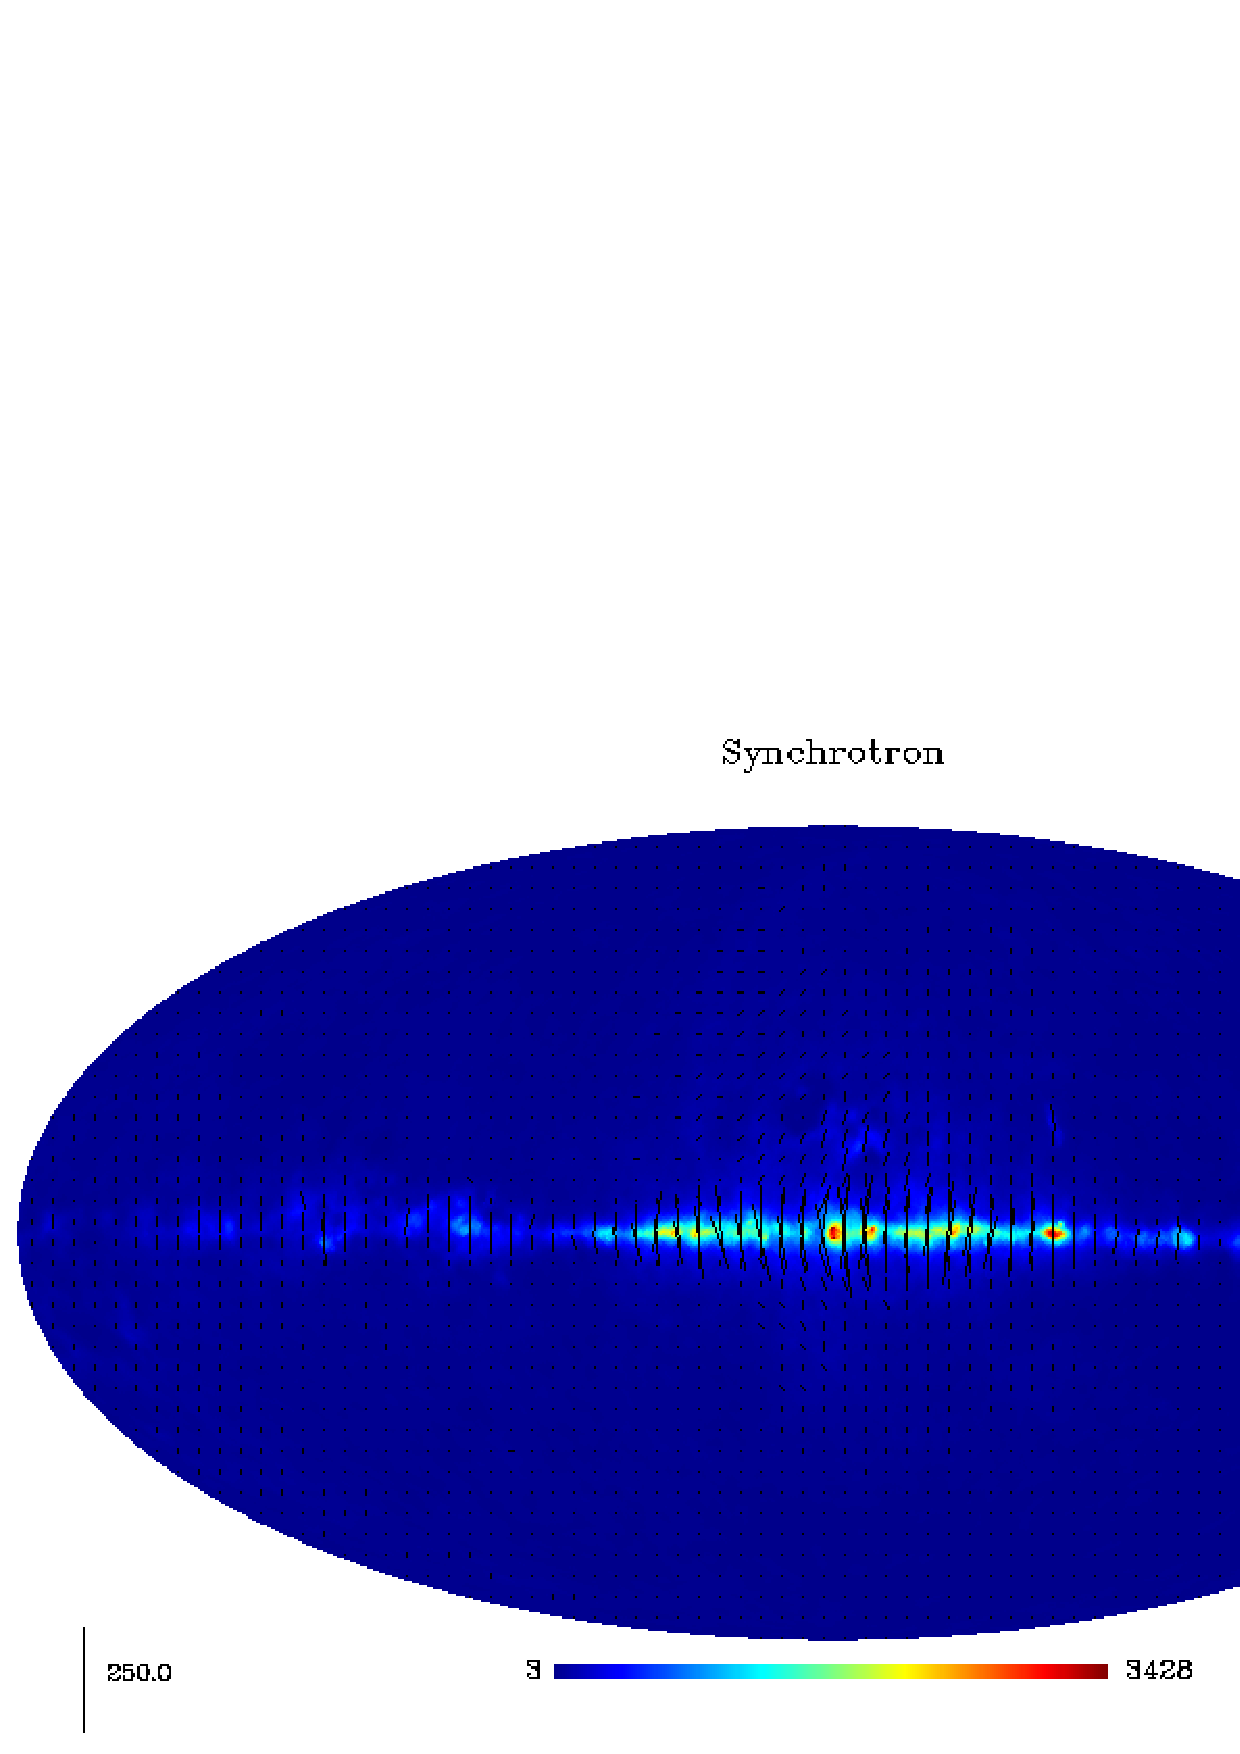
\includegraphics[width=7cm]{fig_mol_synchrotron.pdf}
 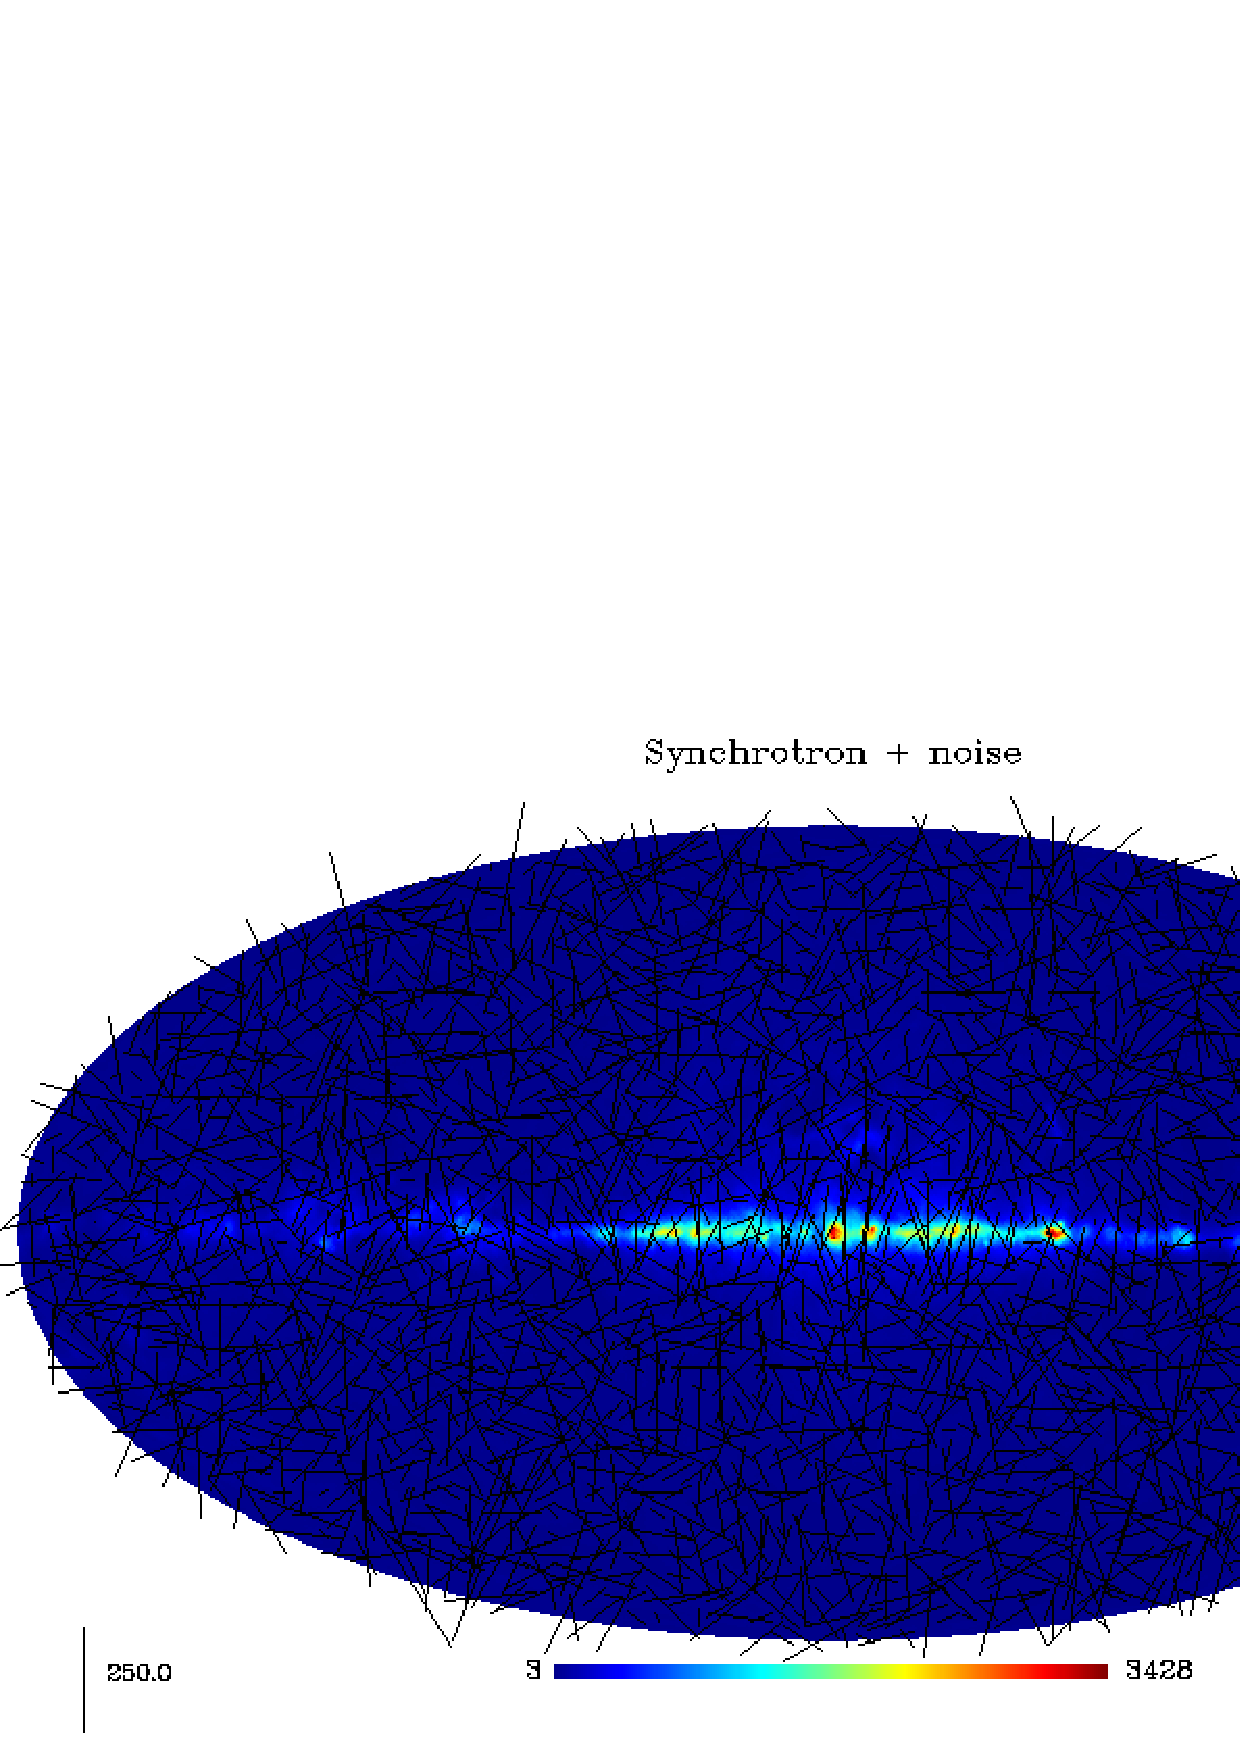
\includegraphics[width=7cm]{fig_mol_synchrotron_noise.pdf}
 }
 }
 \centerline{
 \hbox{
 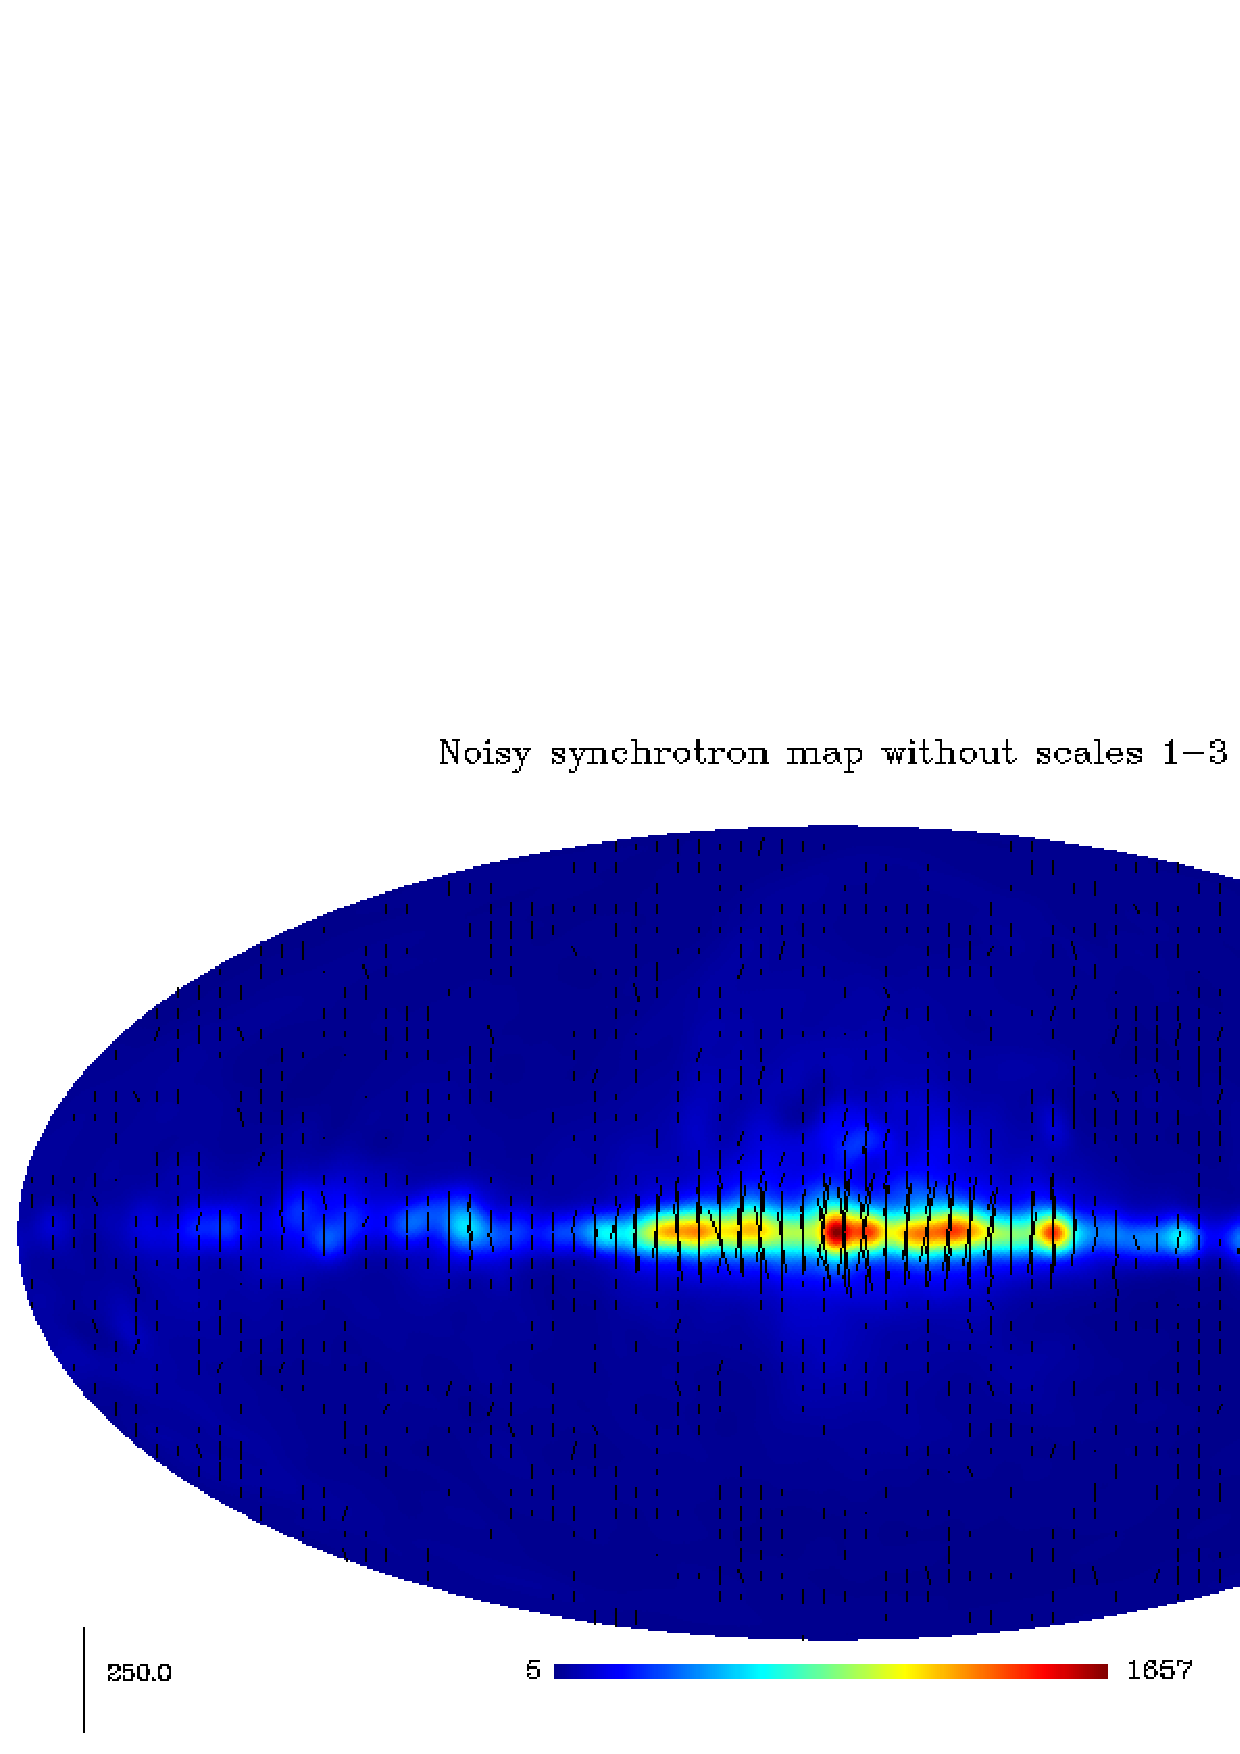
\includegraphics[width=7cm]{fig_mol_synchrotron_noise_no_scale1-3.pdf}
 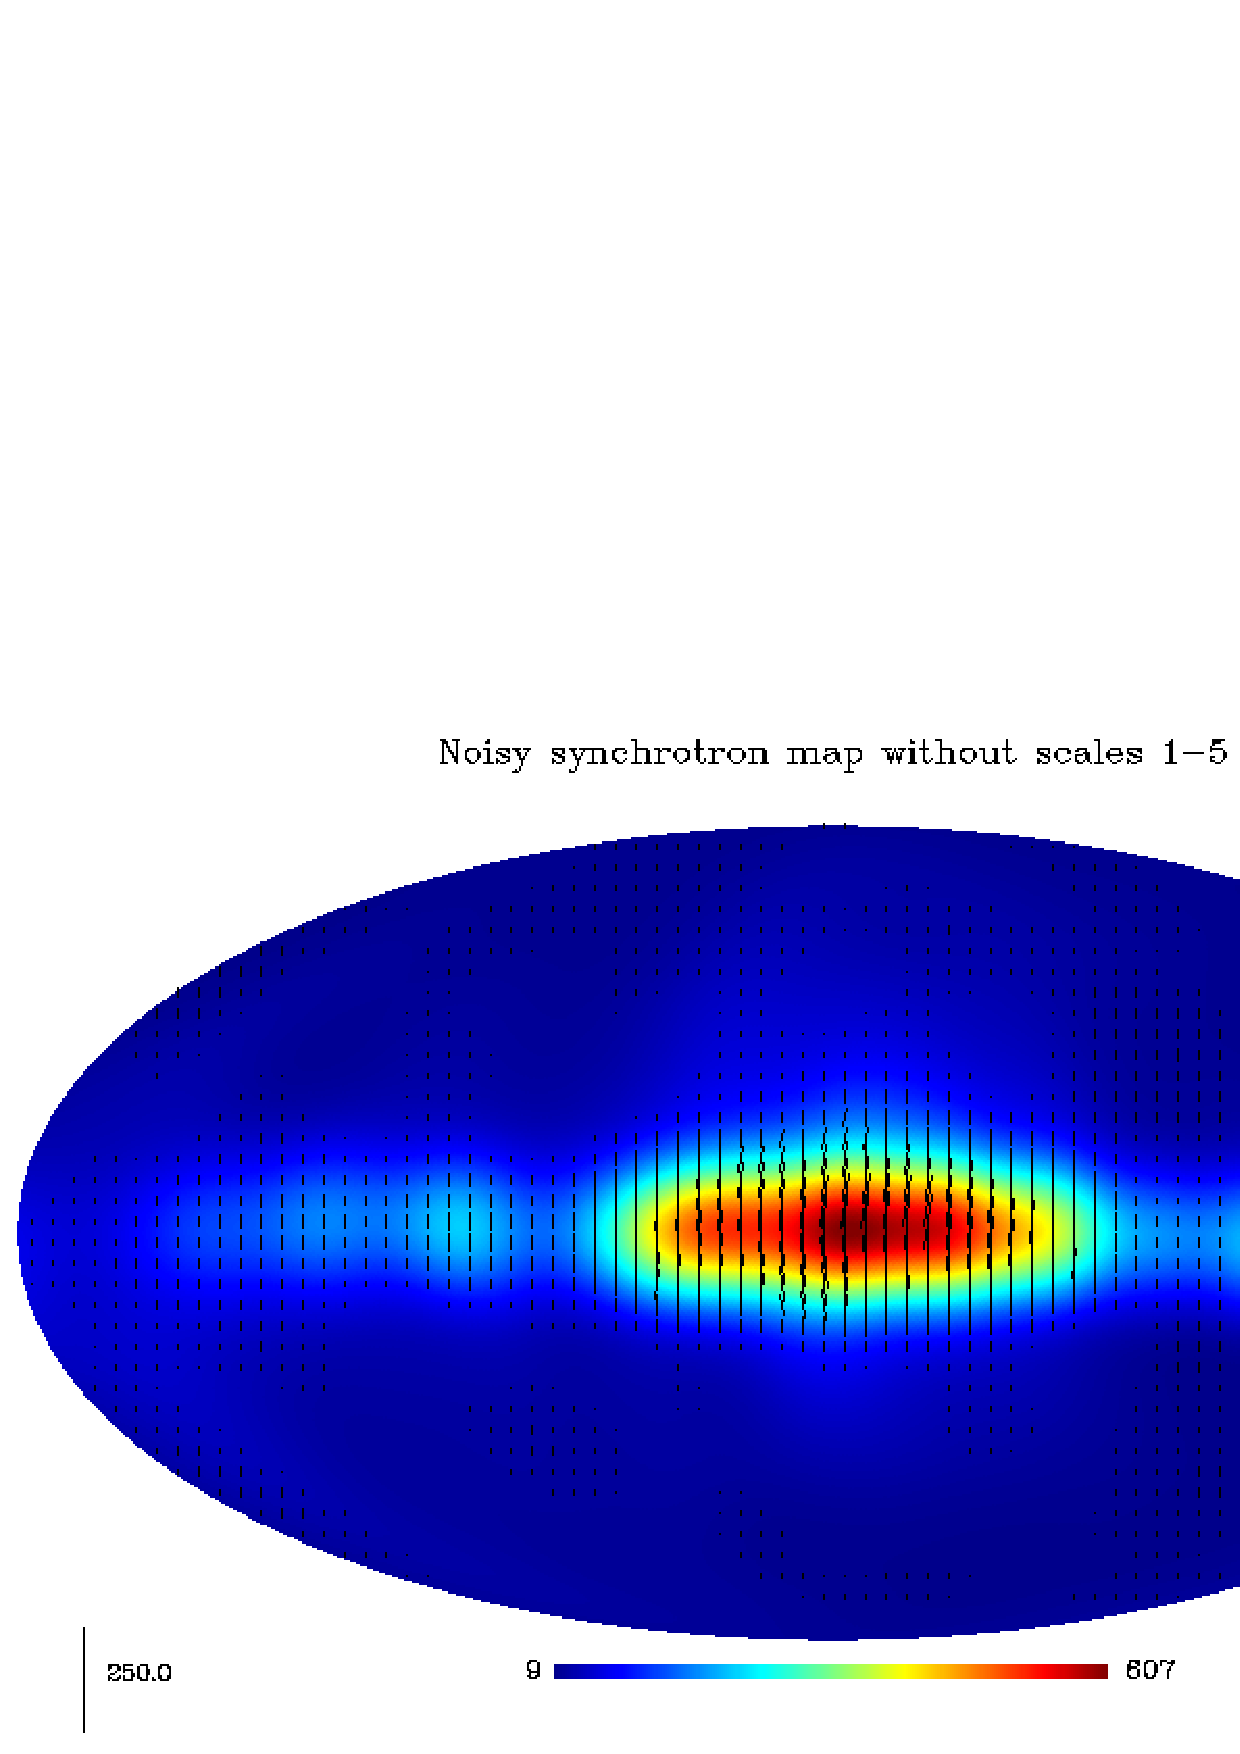
\includegraphics[width=7cm]{fig_mol_synchrotron_noise_no_scale1-5.pdf}
 }
 }
 }
\caption{ Polarized field smoothing - \textit{top left~:} simulated synchroton emission.  \textit{top right~:} same field corrupted by additive noise.
 \textit{bottom left~:} MP-multiscale reconstruction after setting to zero all coefficients from the three first scales.
\textit{bottom right~:} MP-multiscale reconstruction after setting to zero all coefficients from  the five first scales.}
\label{fig_modphase_smoothfield}
\end{figure*}
Fig.~\ref{fig_modphase_smoothfield} top  shows a simulated polarized field of the synchrotron emission and its noisy version.
We have applied the MP-multiscale transform and we remove the first three scales (i.e. we put all coefficients to zero) before 
reconstructing. The resulting image is shown on the bottom left of Fig.~\ref{fig_modphase_smoothfield}. The bottom right of 
Fig.~\ref{fig_modphase_smoothfield} corresponds to the same experiment, but by removing the five first scales. We can see that 
the field is smoother and smoother, but respecting the large scale structure of the field. This transform will be very well suited 
to CMB studies where the phase is analyzed independently of the modulus, such as in~\cite{coles05,naselsky05}.

%---------------------------------------------------------------------------------------------------------------------------------------
%---------------------------------------------------------------------------------------------------------------------------------------


\section{Polarized Wavelet Transform using Spherical Harmonics}
\label{sec:pol_iwt}

\subsection{Isotropic Undecimated Wavelet Transform on the Sphere (UWTS) }
\label{sec:UWTS}

\begin{figure*}[htb]
\centerline{
 \hbox{
 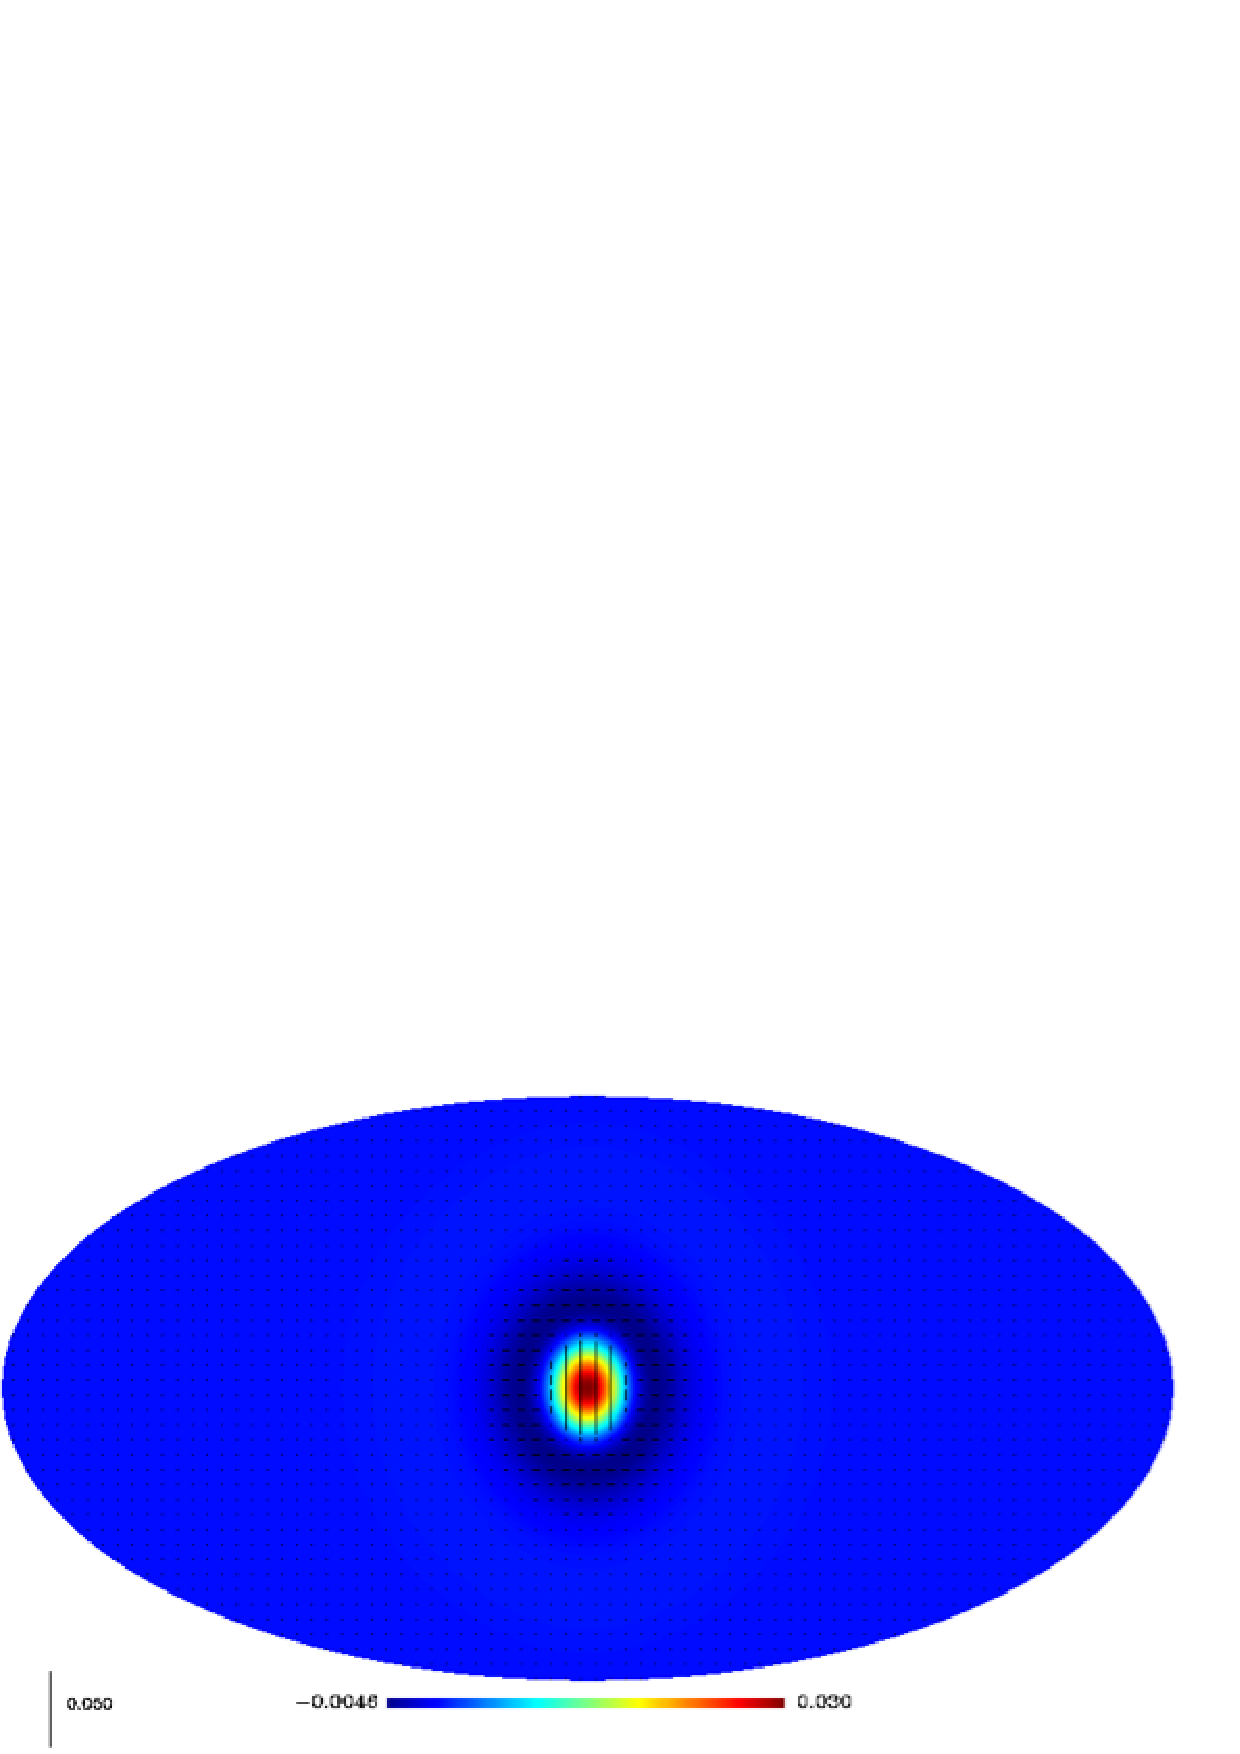
\includegraphics[width=7cm]{fig_q_iwt_back.pdf}
 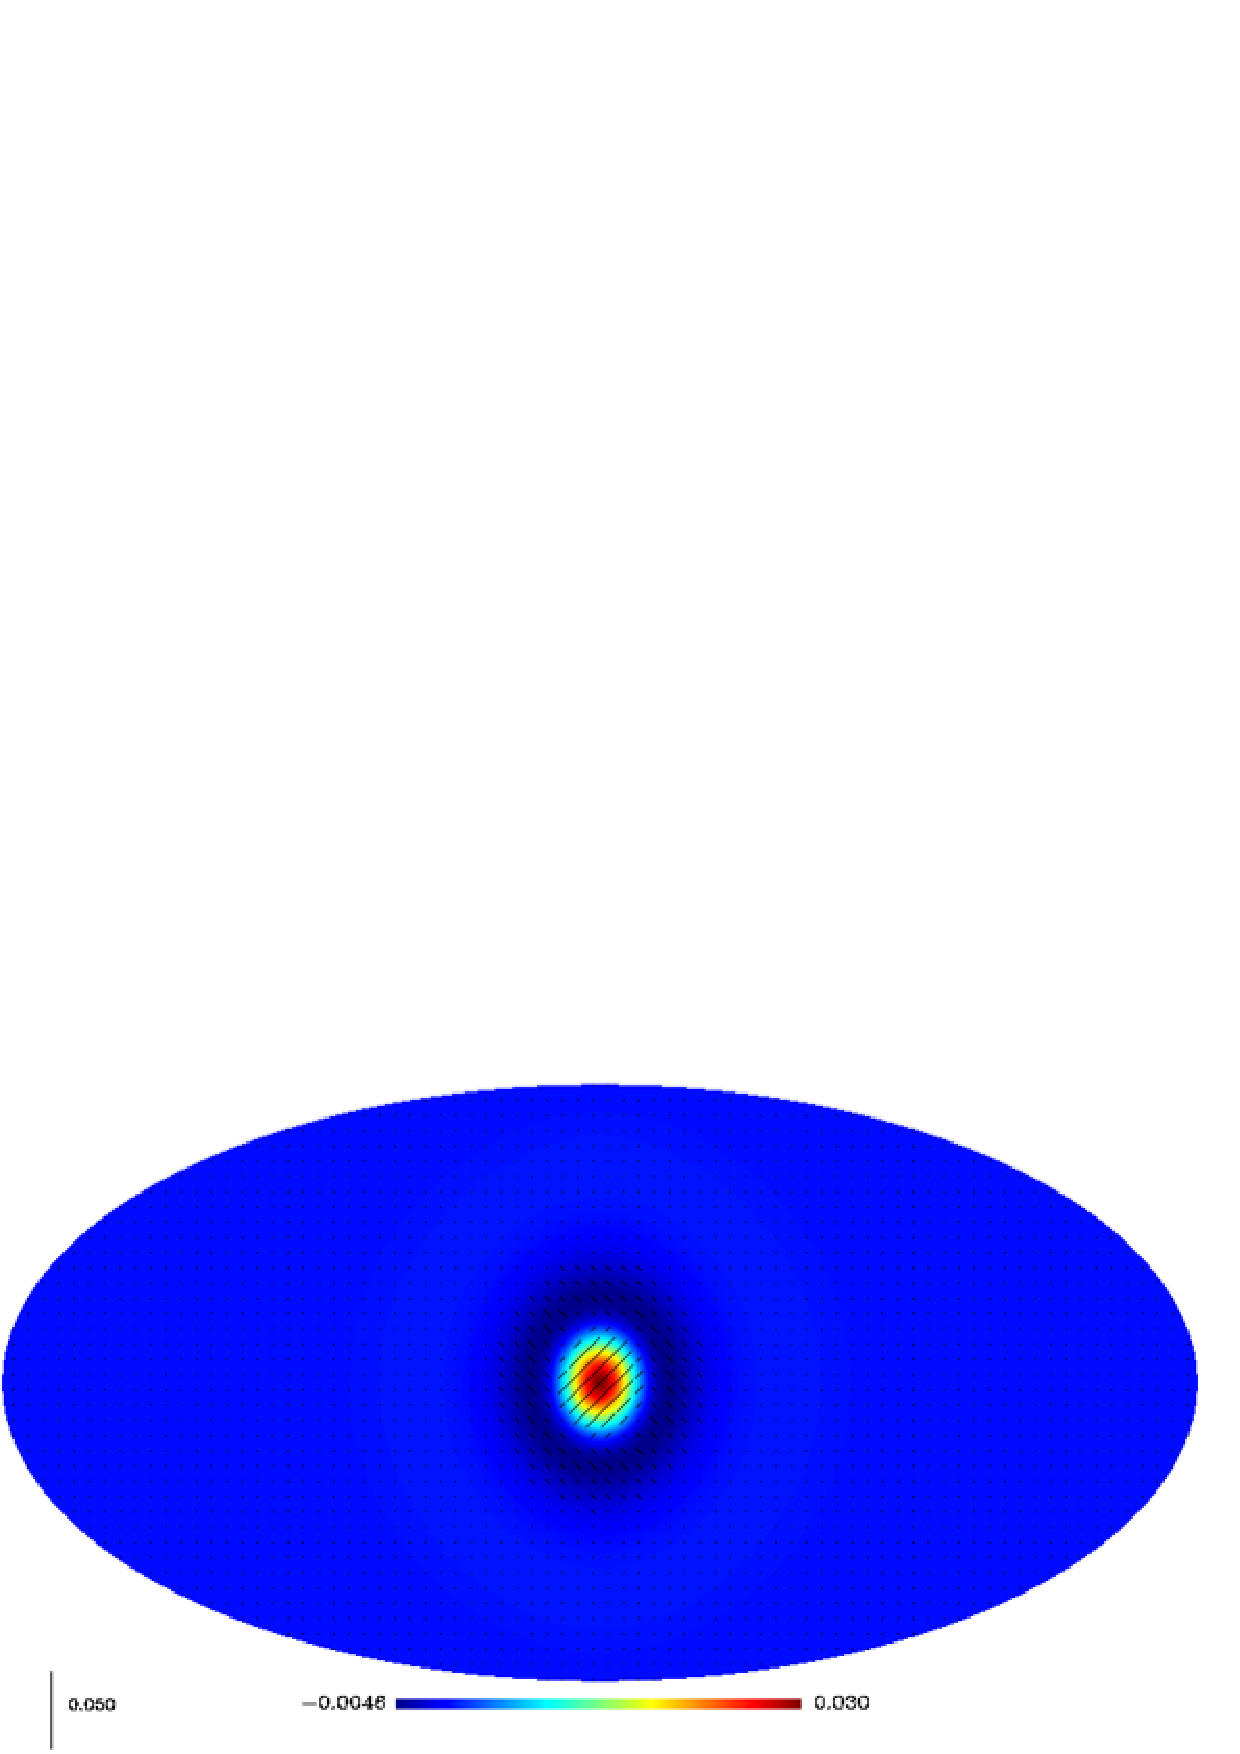
\includegraphics[width=7cm]{fig_u_iwt_back.pdf}
 }
 }
\caption{Q-isotropic wavelet transform backprojection (left) and U-isotropic wavelet backprojection (right).}
\label{fig_qu_iwt_back}
\end{figure*}


%---------------------------------------------------------------------------------------------------------------------------------------
The undecimated isotropic transform on the sphere described in~\cite{starck:sta05_2} is similar in many respects to the usual 
\emph{ \`a trous} isotropic wavelet transform. It is obtained using a zonal scaling function $\phi_{l_c}(\vartheta, \varphi)$ 
which depends only on colatitude $\vartheta$ and is invariant with respect to a change in longitude $\varphi$. It follows that 
the spherical harmonic coefficients $\hat \phi_{l_c} (l,m)$ of $\phi_{l_c}$ vanish when $m \ne 0$ which makes it simple to compute 
those spherical harmonic coefficients $\hat c_{0}(l,m)$ of $c_0 = \phi_{l_c} * f$ where $*$ stands for convolution :
\begin{eqnarray}
 \hat c_{0}(l,m) = \widehat{\phi_{l_c} * f} (l,m) = \sqrt{\frac{4\pi}{2l+1} } \hat \phi_{l_c} (l,0) \hat f(l,m) 
\end{eqnarray}
A possible scaling function~\cite{starck:book98}, defined in the spherical harmonics representation, is $\phi_{l_c}(l, m) = {2 \over 3} B_{3} ( { {2 l} \over {l_{c} } } )$ 
where $B_{3}$ is the cubic B-spline compactly supported over $[-2, 2]$. Denoting $\phi_{2^{-j} l_{c} }$ a rescaled version of 
$\phi_{l_{c}}$ with cut-off frequency $2^{-j} l_{c}$, a multi-resolution decomposition of $f$ on a dyadic scale is obtained recursively : 
\begin{eqnarray}
c_0   & = &  \phi_{ l_{c} }  * f    \nonumber    \\
c_j    &=&   \phi_{2^{-j}  l_{c}  }  * f  =   c_{j-1} * h_{j-1} \nonumber    \\
\end{eqnarray}
where the zonal low pass filters $h_{j}$ are defined by 
\begin{eqnarray}
 \hat{H}_{j}(l,m)  & =  &  \sqrt{\frac{4\pi}{2l+1} }  \hat h_{j}(l,m)  \nonumber \\
 &  =  & \left\{
  \begin{array}{ll}
  \frac {   \hat \phi_{\frac{l_{c}}{2^{j+1}} }(l,m)   }   {  \hat  \phi_{  \frac{l_{c}}{2^{j}} }(l,m)   } & \mbox{if }  l  < \frac{ l_{c}} {2^{j+1}} \quad \textrm{and}\quad m = 0\\
0 & \mbox{otherwise } \ 
  \end{array}
  \right.
\end{eqnarray}
The cut-off frequency is reduced by a factor of $2$ at each step so that in applications where this is useful such as compression, 
the number of samples could be reduced adequately. Using a pixelization scheme such as Healpix \cite{pixel:healpix}, this can easily 
be done by dividing by 2 the Healpix {\it nside} parameter when computing the inverse spherical harmonics transform. 
% Of course, this is only an approximate \emph{Sampling Theorem} but it proved sufficient for numerical purposes.  However, in the present isotropic undecimated transform, no downsampling is performed  and the maps have the same number of pixels on each scale. Hence the orthogonality requirement is relaxed, which provides us with a higher degree of freedom in the choice and design  of the wavelet function $\psi_{l_c}$ to be used with the scaling function $\phi_{l_c}$. 
As in the \emph{\`a trous} algorithm, the wavelet coefficients can be defined as the difference between two consecutive resolutions, 
$w_{j+1}(\vartheta, \varphi) = c_{j}(\vartheta, \varphi) - c_{j+1}(\vartheta, \varphi)$. This defines a zonal wavelet function $\psi_{l_c}$ as 
\begin{eqnarray}\label{wavelet}
\hat \psi_{\frac{l_c}{2^{j}}}(l,m) = \hat \phi_{\frac{l_c}{2^{j-1}}} (l,m)  - \hat \phi_{\frac{l_c}{2^{j}}}(l,m)
\end{eqnarray}

\begin{figure*}[htb]
\centerline{
\hbox{
 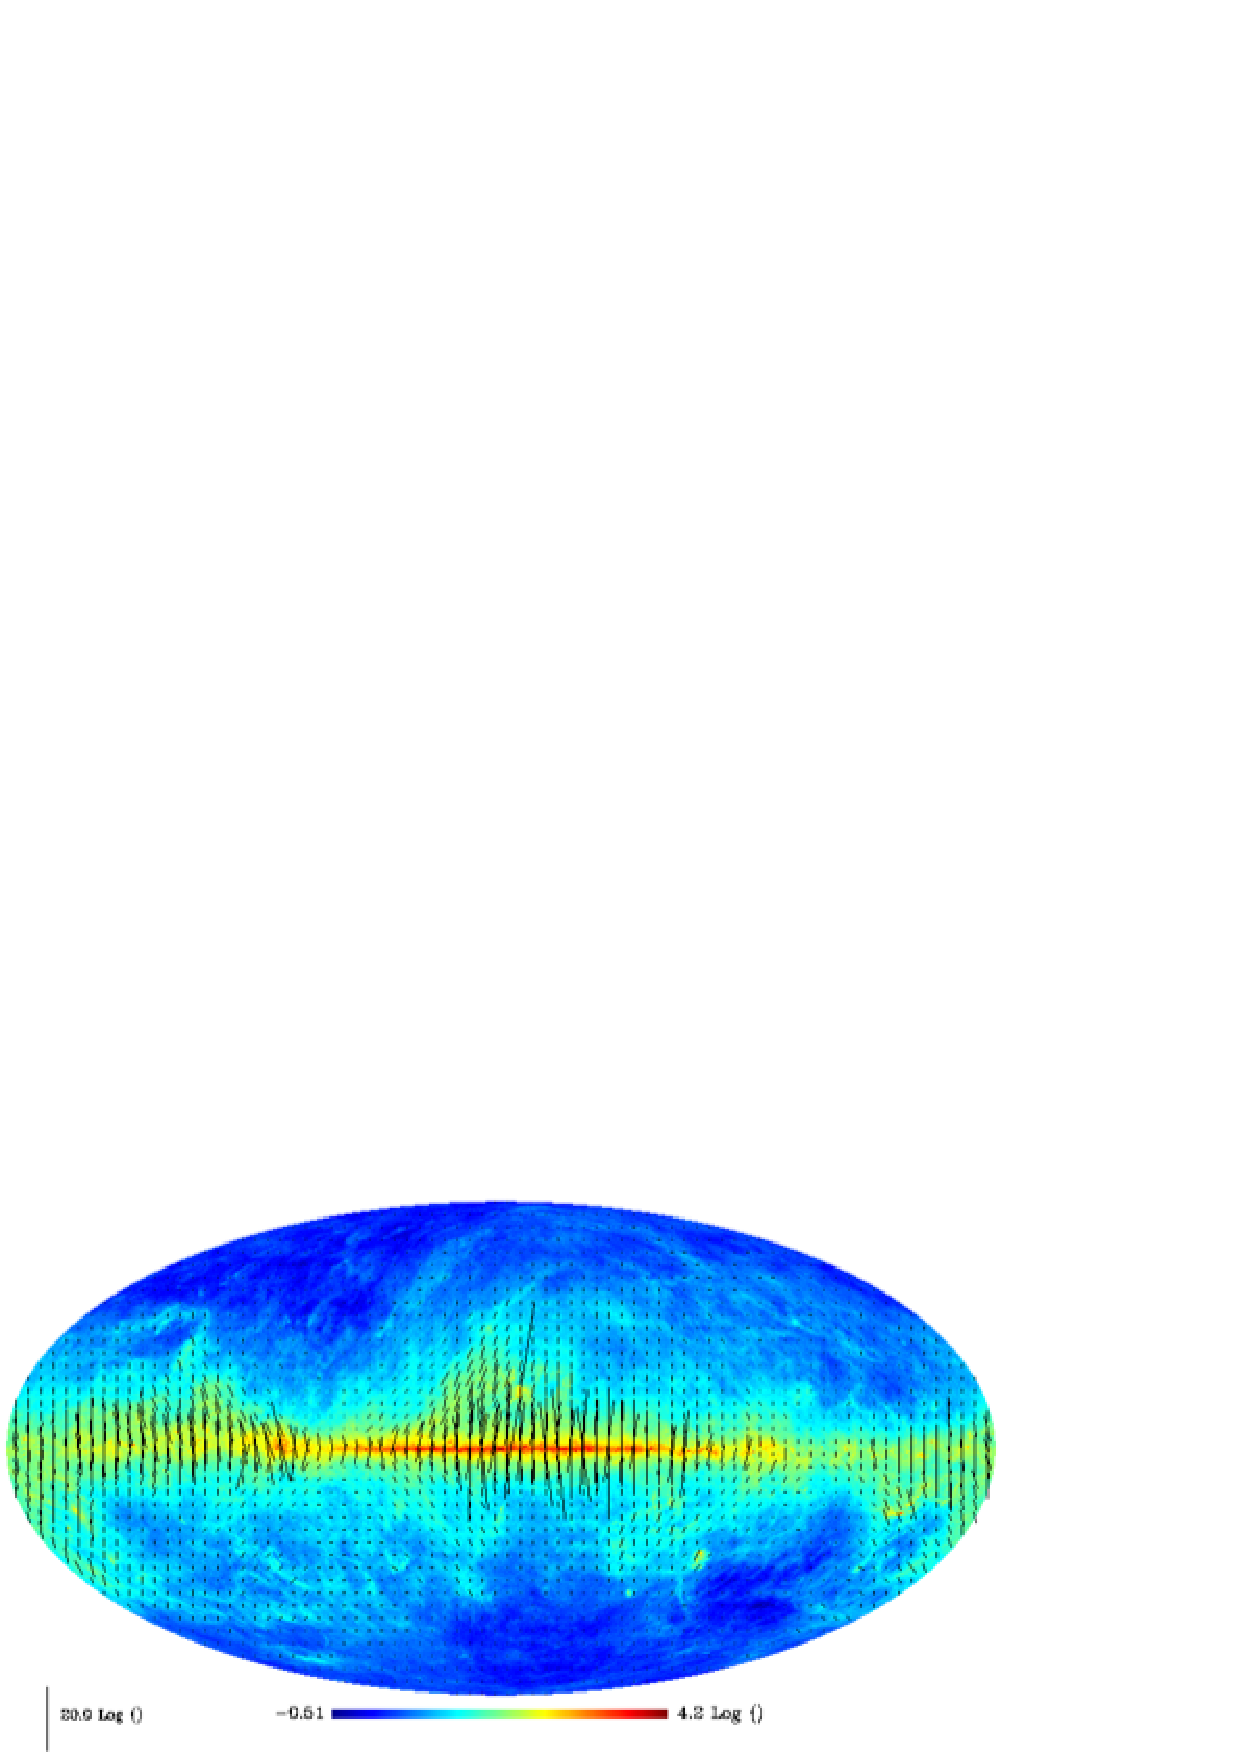
\includegraphics[width=7cm]{fig_dust_input.pdf}
}}
\caption{Simulated observations on the sphere of the polarized galactic dust emission.}
\label{fig_simu_pol_dust}
\end{figure*}

With this particular choice of wavelet function, the decomposition is readily inverted by summing the coefficient maps on all wavelet scales
 \begin{eqnarray}\label{IWT}
   %c_{0}(\vartheta, \varphi) = c_{J}(\vartheta, \varphi) + \sum_{j=1}^{J} w_j(\vartheta, \varphi)
   f(\vartheta, \varphi) = c_{J}(\vartheta, \varphi) + \sum_{j=1}^{J} w_j(\vartheta, \varphi)
\end{eqnarray}
where we have made the simplifying assumption that $f$ is equal to $c_0$. Obviously, other wavelet functions $\psi$ could be used just as well, such as the needlet function~\cite{marinucci08}.

% Also,  because of the redundancy of the described decomposition, the inverse transform  is not unique and in fact this can profitably be used to impose additional constraints on the synthesis functions (\emph{e.g.} smoothness, positivity) used in the reconstruction \cite{starck:sta06}. 

\begin{figure*}[htb]
\centerline{
\vbox{
 \hbox{
 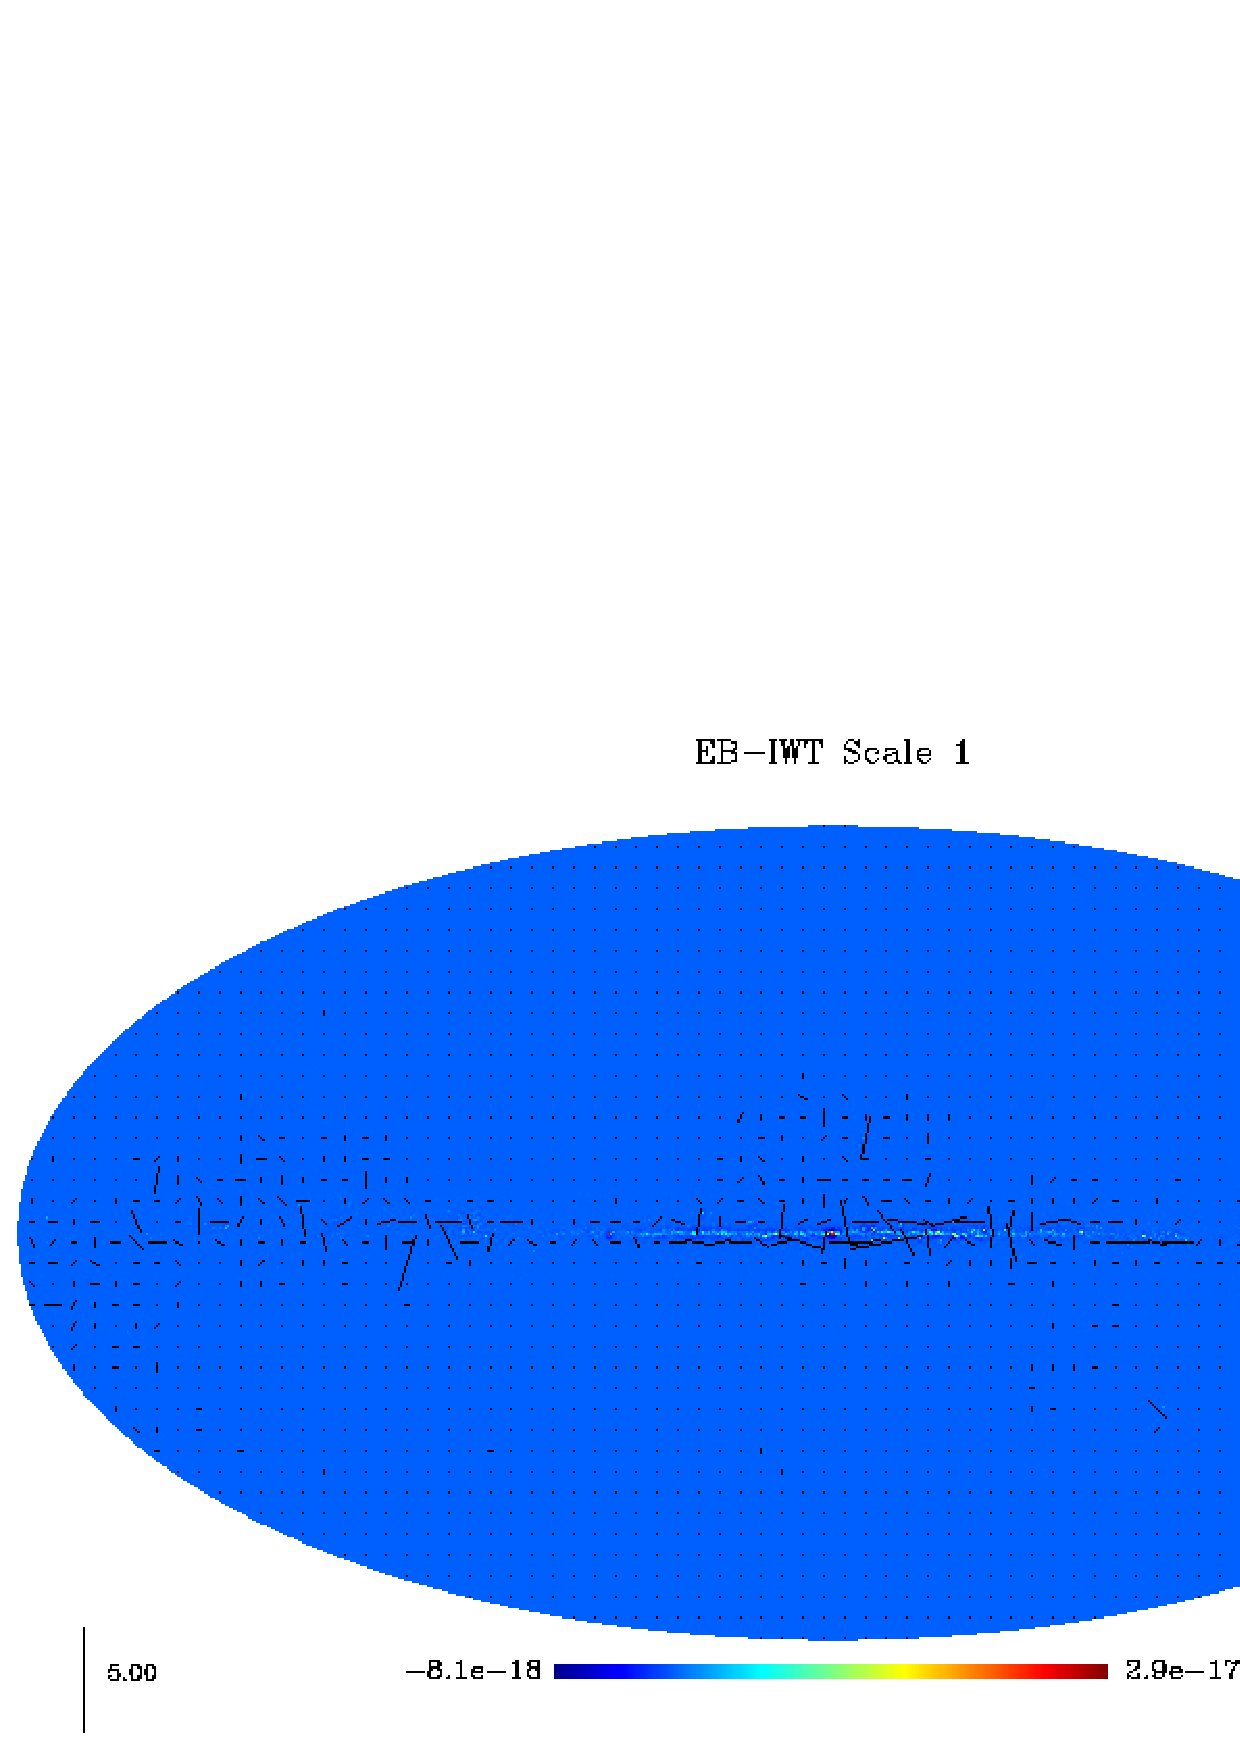
\includegraphics[width=7cm]{fig_ebiwt_scale1.pdf}
 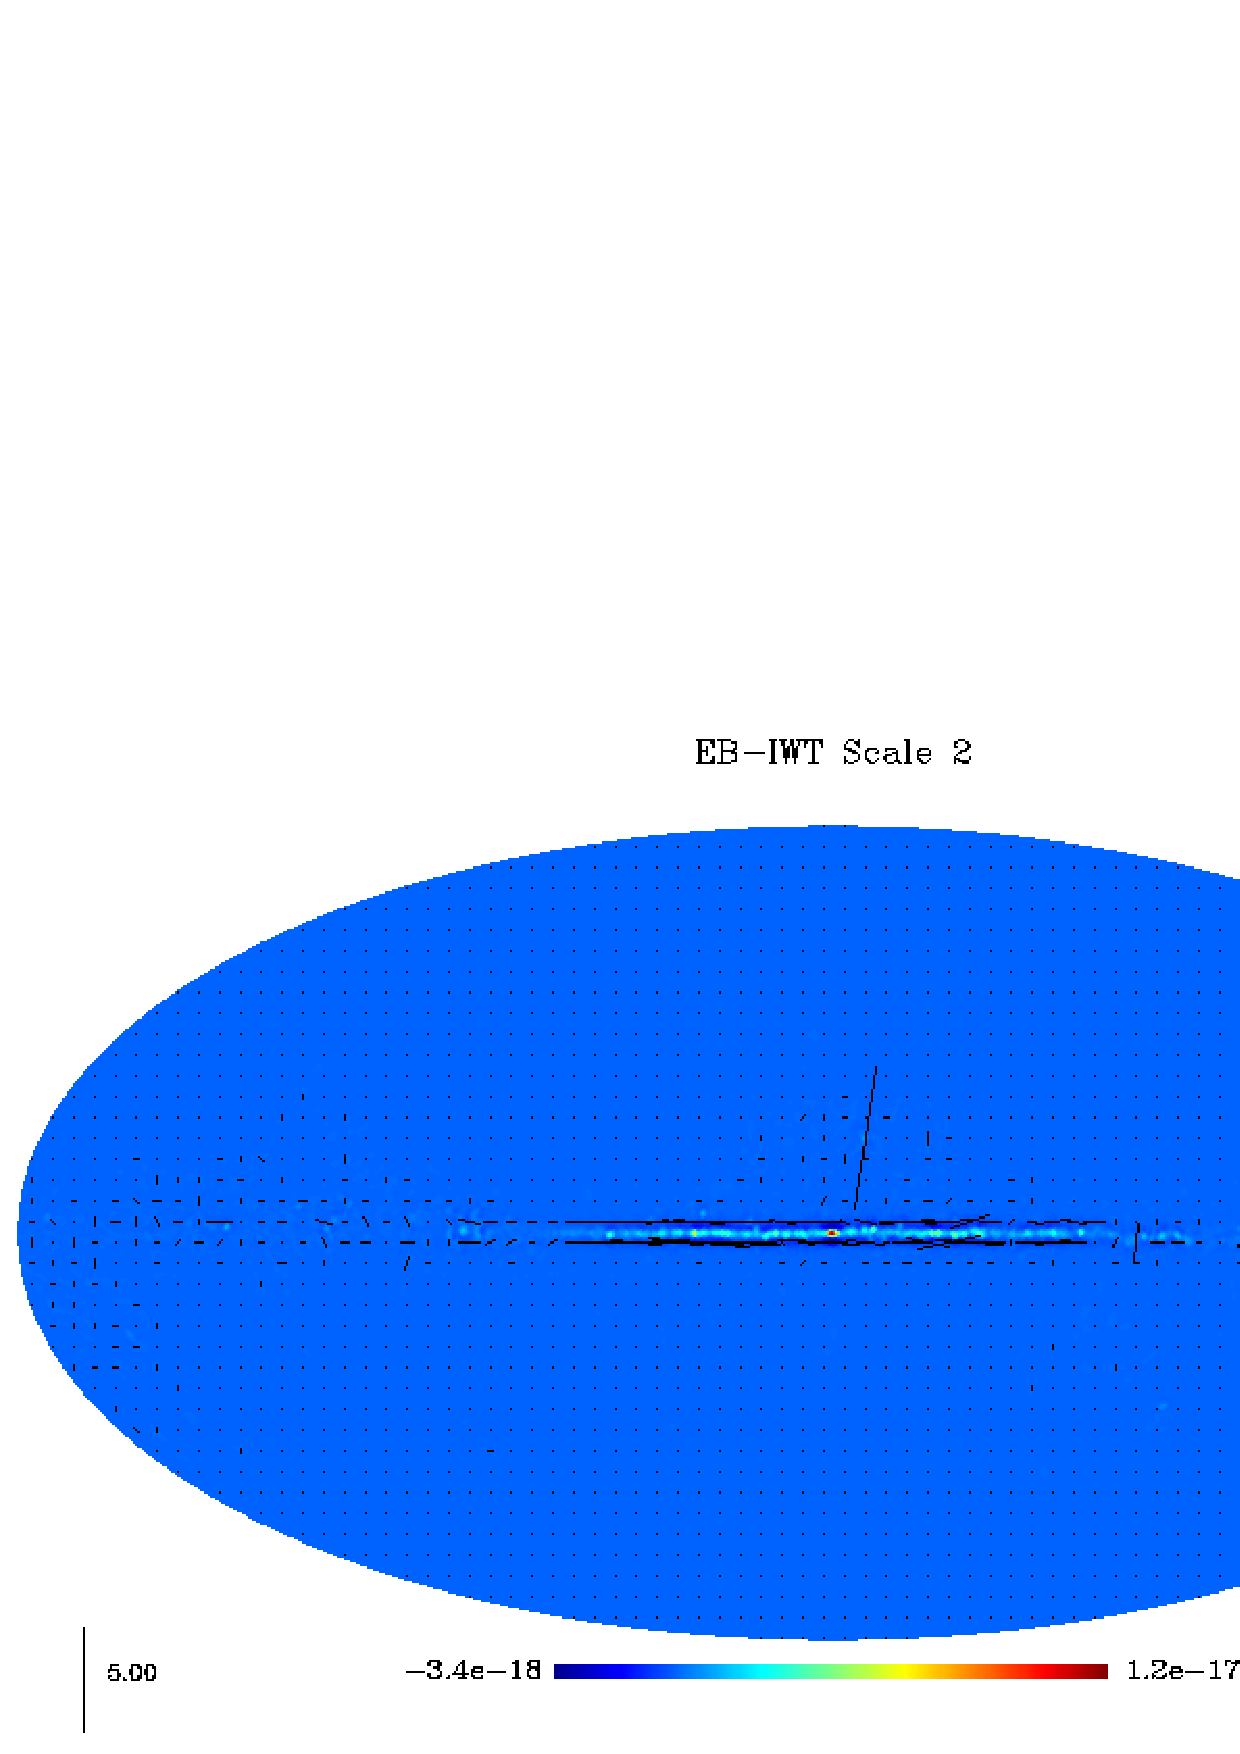
\includegraphics[width=7cm]{fig_ebiwt_scale2.pdf}
 }
 \hbox{
 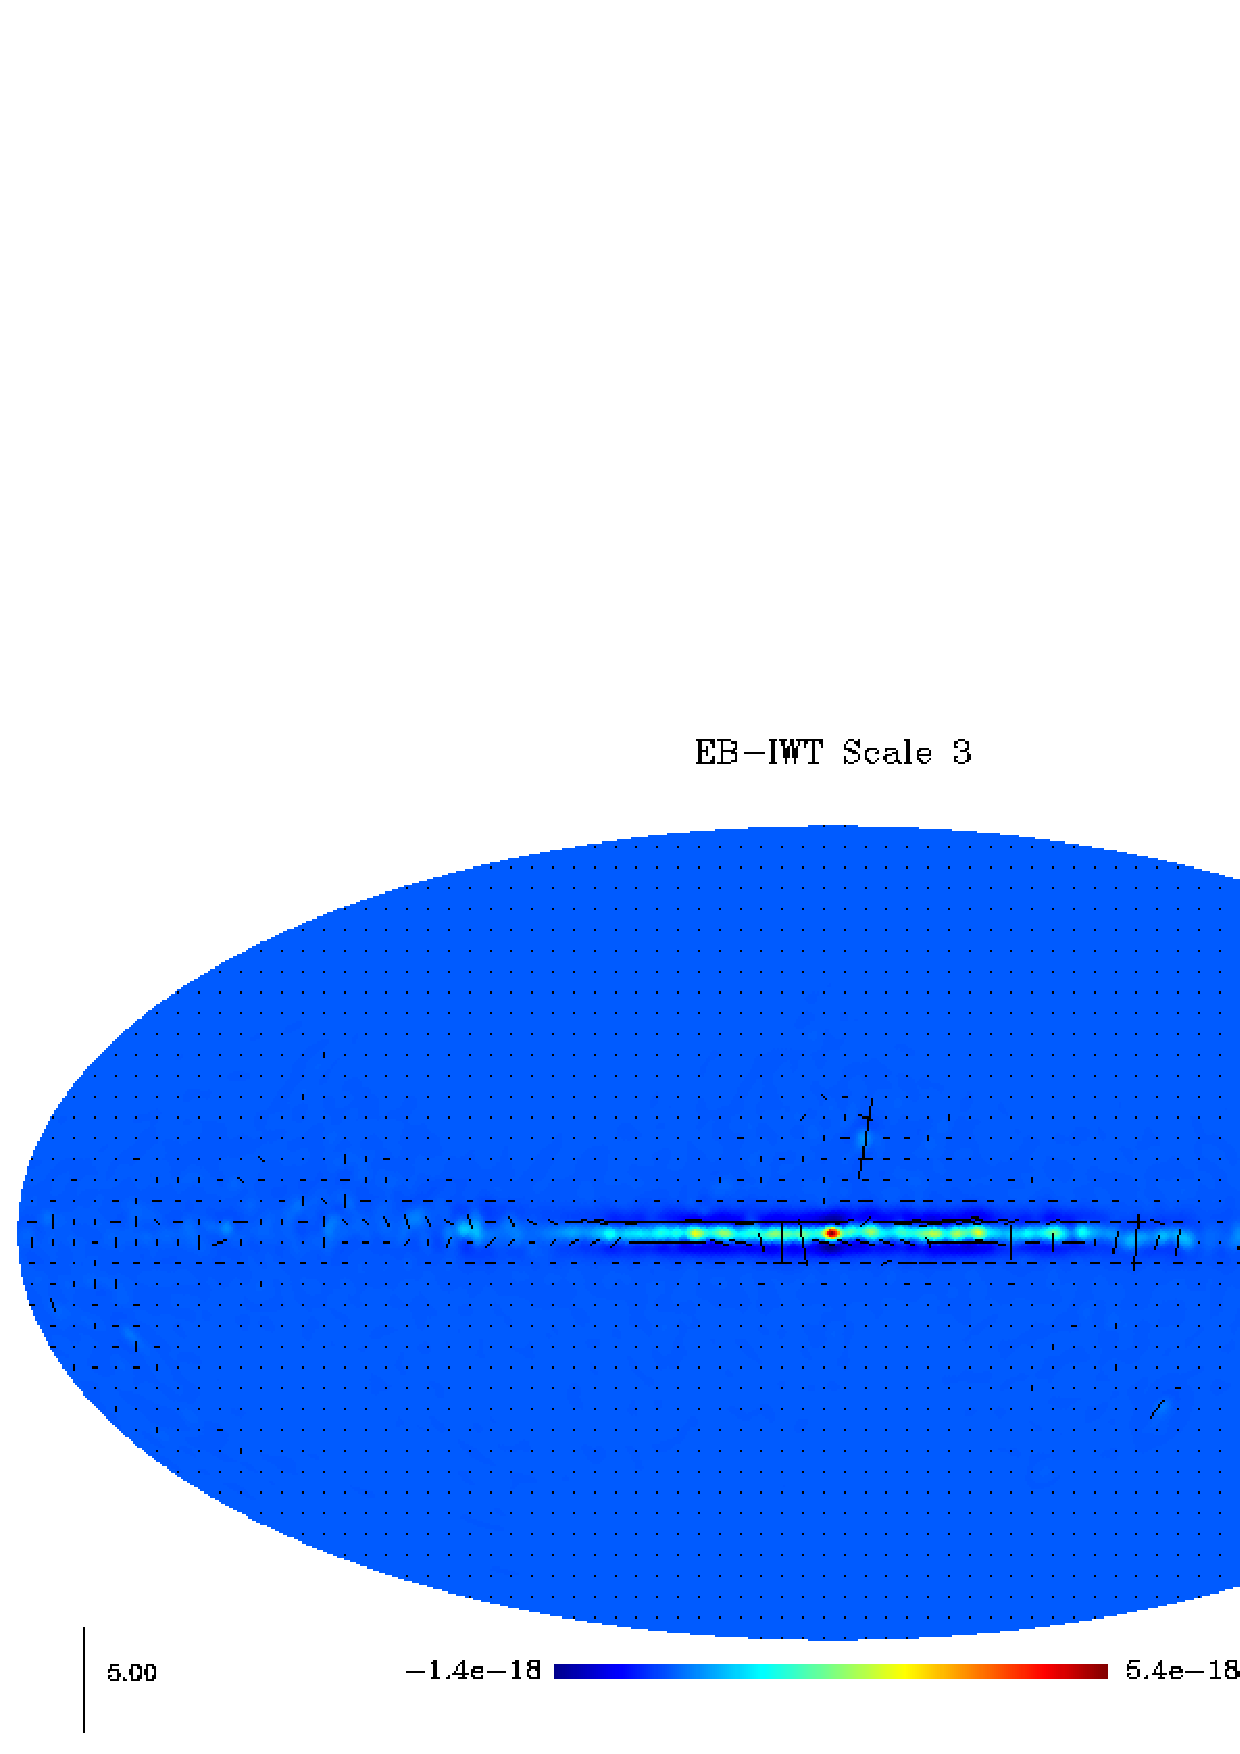
\includegraphics[width=7cm]{fig_ebiwt_scale3.pdf}
 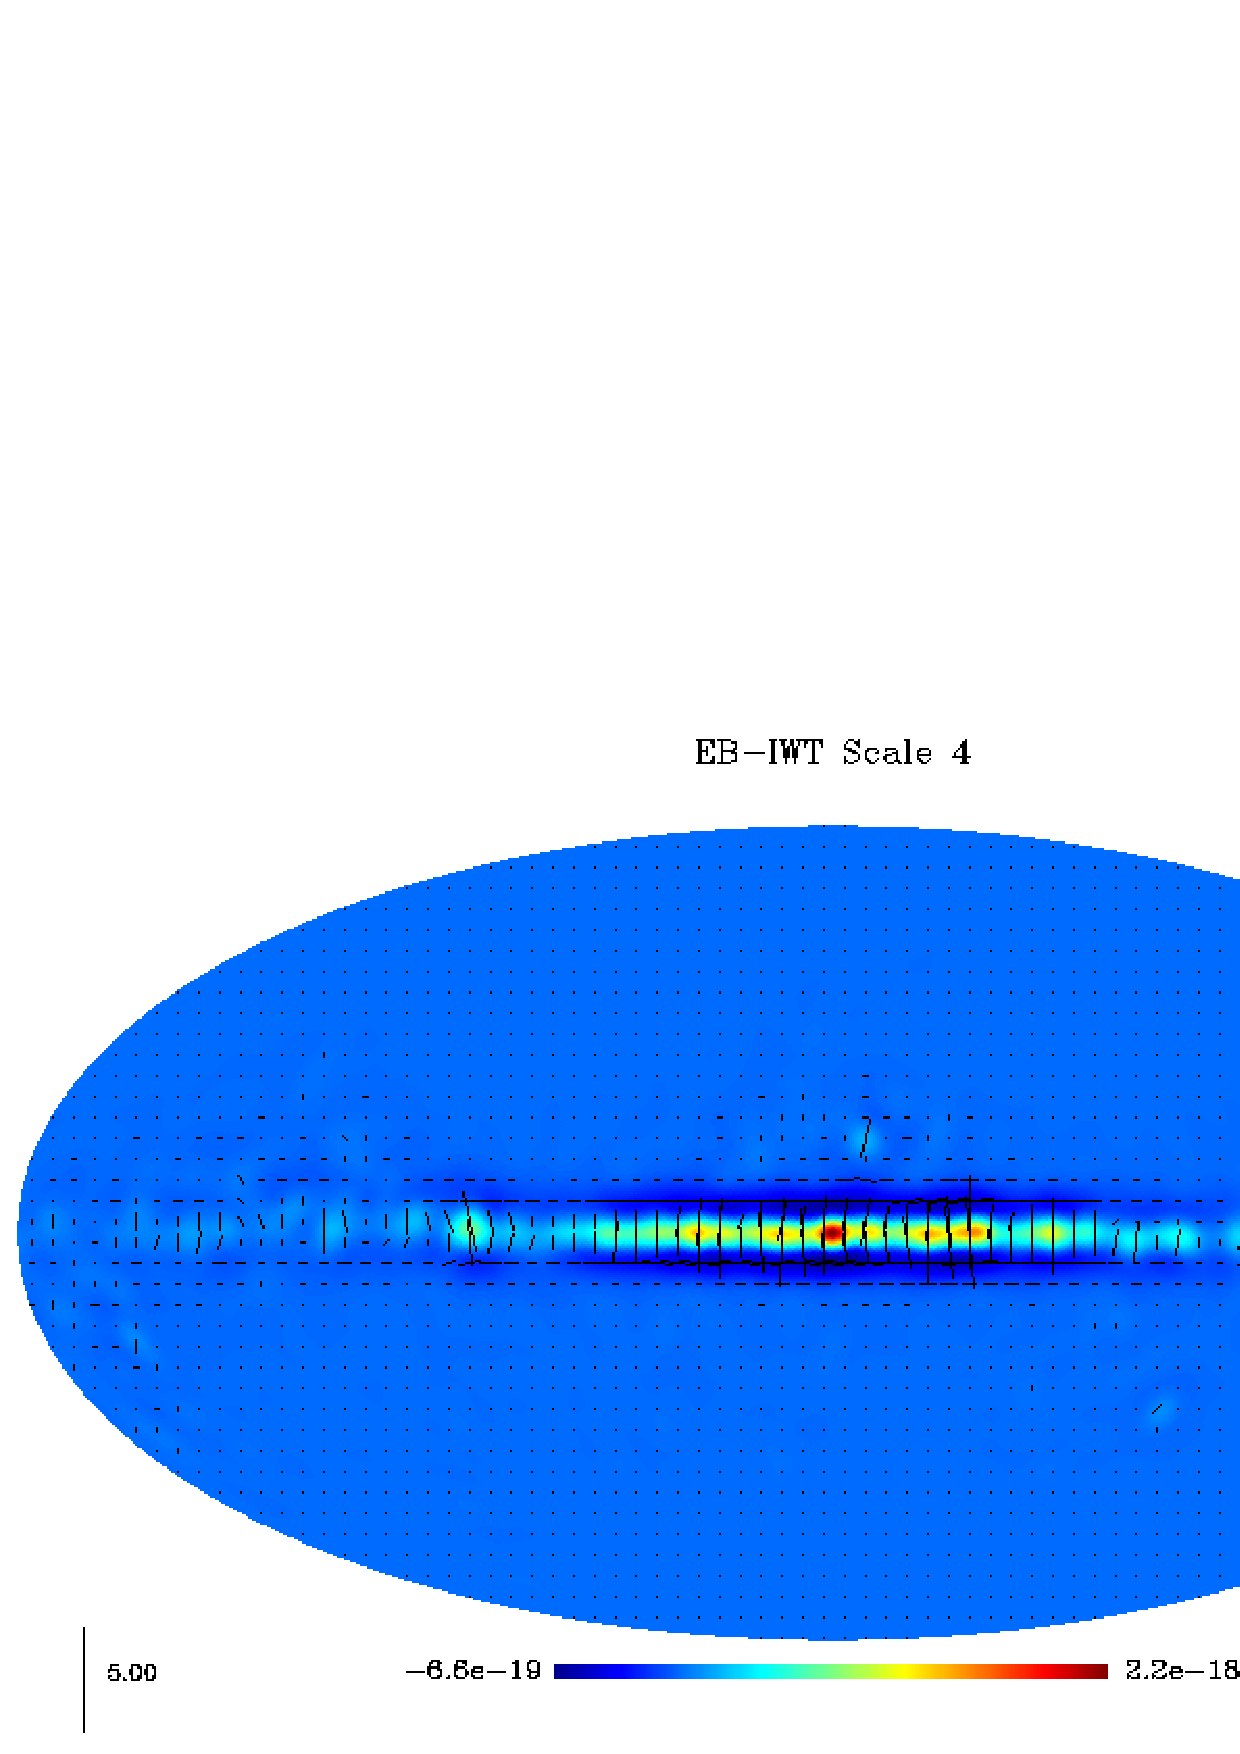
\includegraphics[width=7cm]{fig_ebiwt_scale4.pdf}
 }
  \hbox{
 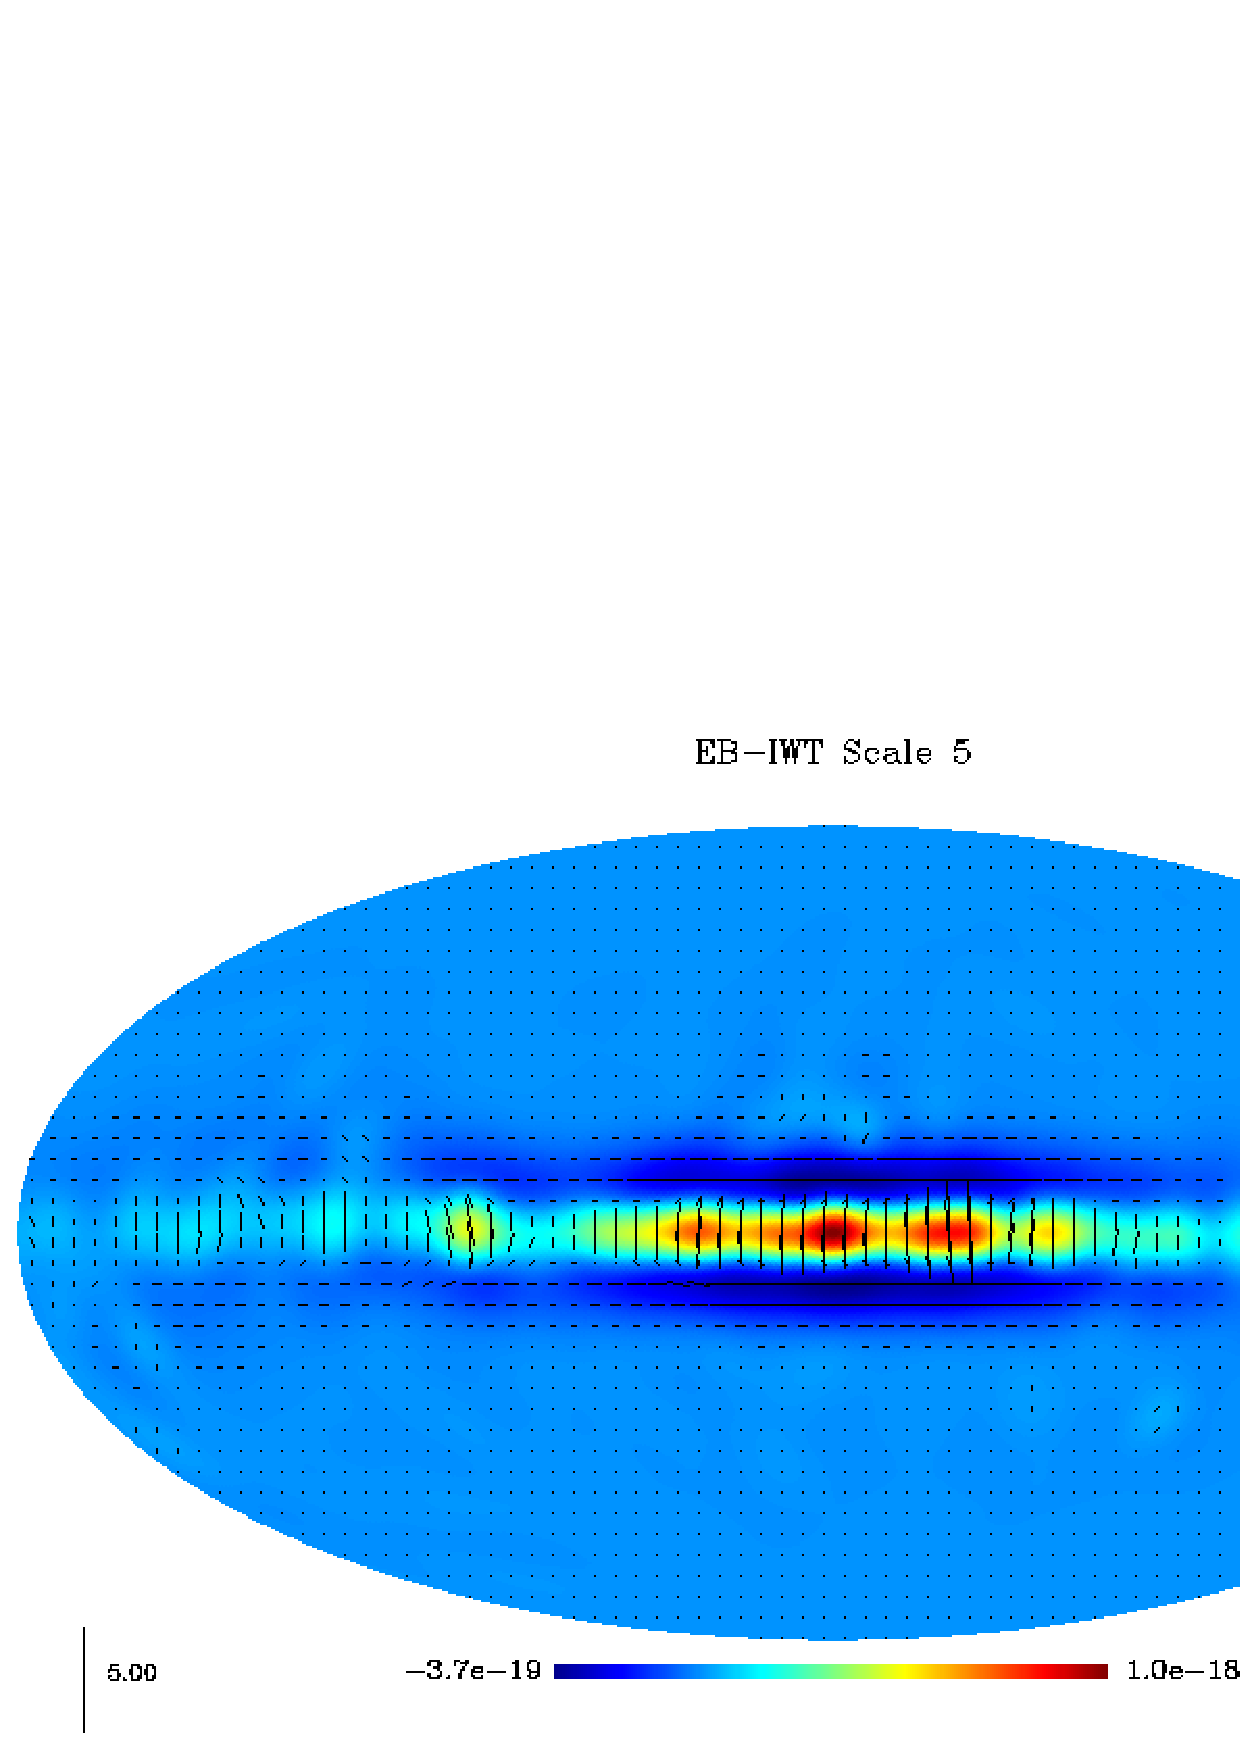
\includegraphics[width=7cm]{fig_ebiwt_scale5.pdf}
 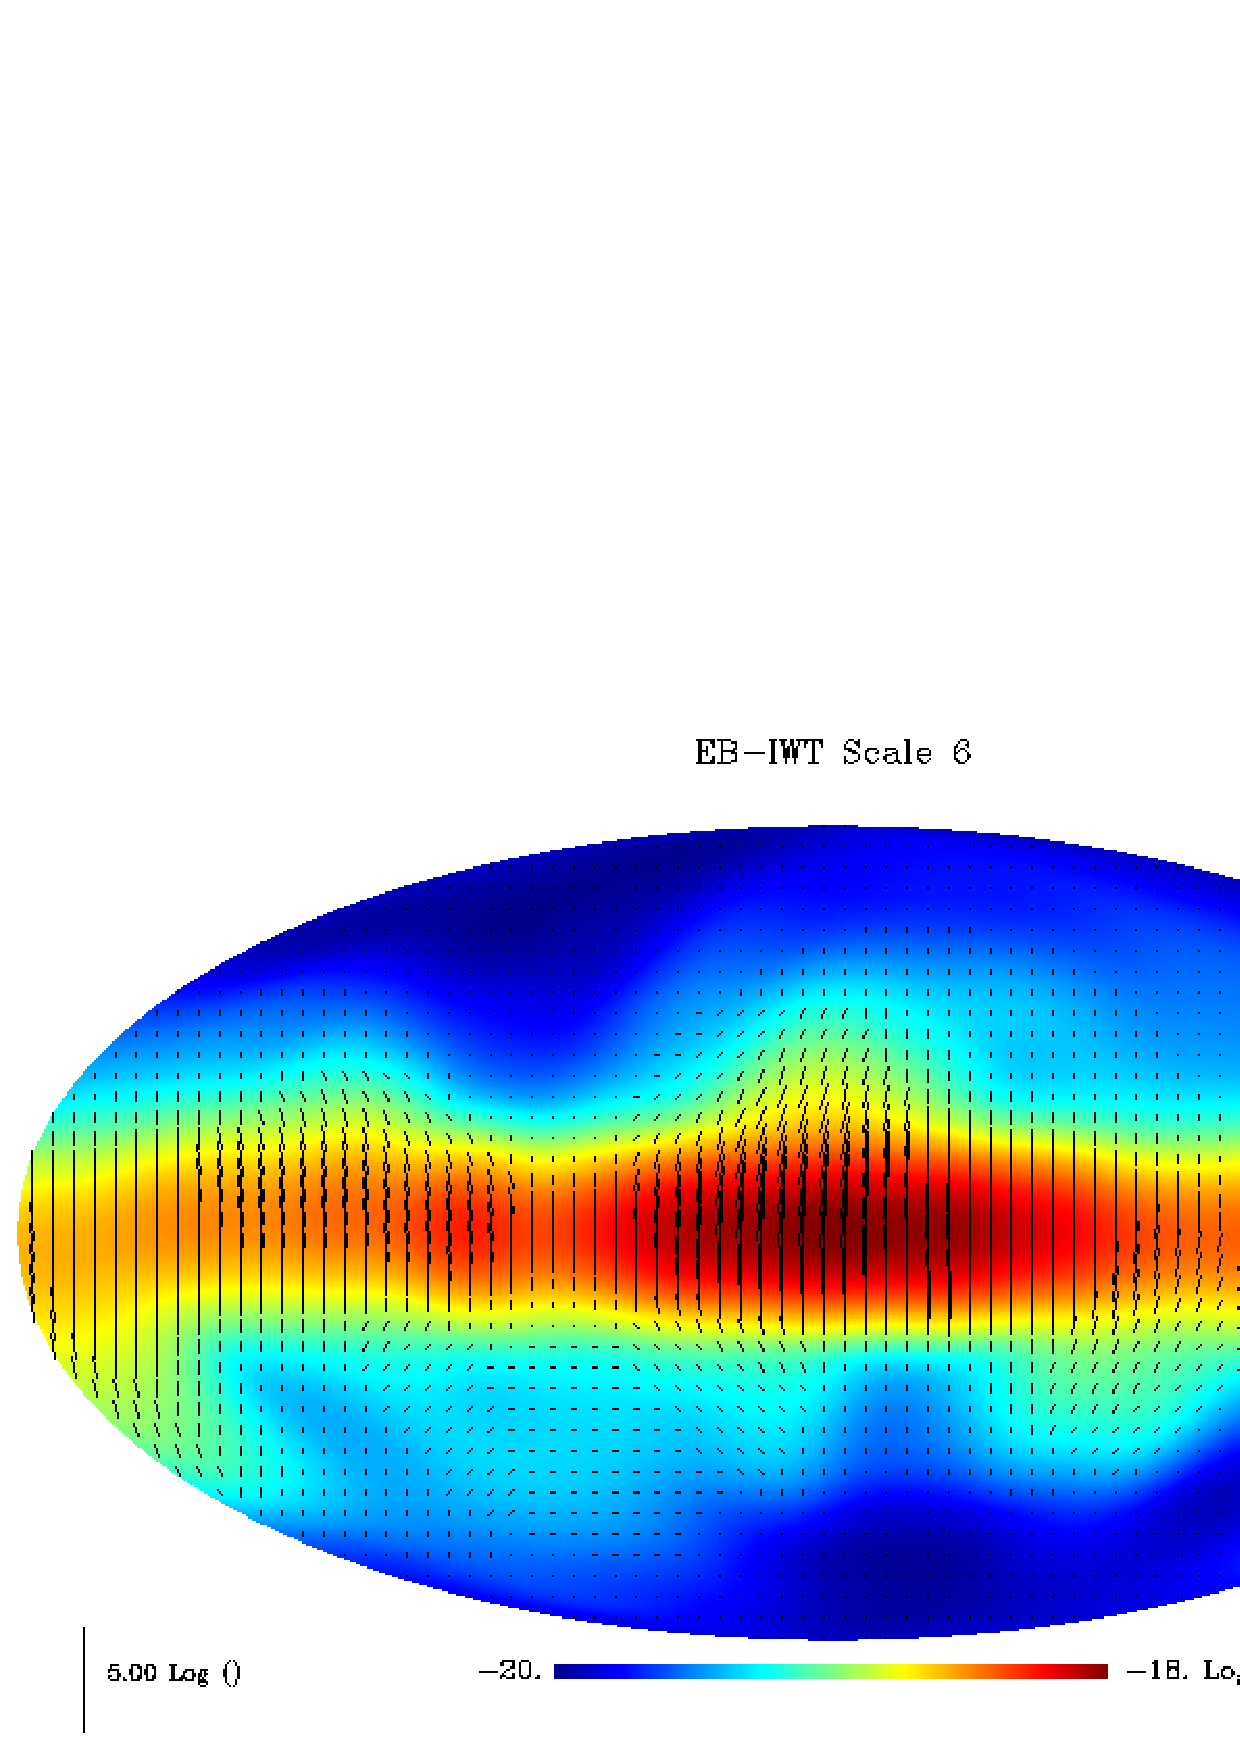
\includegraphics[width=7cm]{fig_ebiwt_scale6.pdf}
 }
  }
 }
\caption{QU-Undecimated Wavelet Transform of the simulated polarized map of galactic dust emission shown in figure~(\ref{fig_simu_pol_dust}).}
\label{fig_quwt_trans_dust}
\end{figure*}

\subsection{Extension to Polarized Data}
By applying the above scalar isotropic wavelet transform to each component $T$, $Q$, $U$ of a polarized map on the sphere, we have~:
\begin{eqnarray}
\label{tqu_iwt}
T(\vartheta, \varphi) & = c_{J}^T (\vartheta, \varphi)+ \sum_{j=1}^{J} w_j^T  (\vartheta, \varphi)\\ \nonumber
Q(\vartheta, \varphi) & = c_{J}^Q (\vartheta, \varphi)+ \sum_{j=1}^{J} w_j^Q (\vartheta, \varphi)\\ \nonumber
U(\vartheta, \varphi) & = c_{J}^U (\vartheta, \varphi)+ \sum_{j=1}^{J} w_j^U (\vartheta, \varphi)
\end{eqnarray}
where $c_{J}^X$ stands for the low resolution approximation to component $X$ and $w_j^X$ is the map of wavelet coefficients of that component on scale $j$. This leads to the following decomposition~:
\begin{eqnarray}
(Q \pm iU)[k] =    (c^Q_{J} \pm c^U_{J,p})[k]   +   \sum_{j=1}^J   ( w_{j}^Q \pm w_{j}^U )[k]
\label{eq_qu_rec_uwt}
\end{eqnarray}
Fig.\ref{fig_qu_iwt_back} shows the backprojection of a Q-wavelet coefficient (left) and a $U$-wavelet coefficient (right).
Fig.~\ref{fig_quwt_trans_dust} shows the undecimated isotropic polarized wavelet transform of the dust image shown on 
Fig.~\ref{fig_simu_pol_dust} using six scales, \textit{i.e.} five wavelet scales and the coarse approximation.
%---------------------------------------------------------------------------------------------------------------------------------------
%---------------------------------------------------------------------------------------------------------------------------------------
\section{Polarized Curvelet Transform}
\label{sec:pol_cur}
% \begin{figure*}
% \centerline{
% \hbox{
% \psfig{figure=fig_back_cur_sphere.ps,bbllx=1cm,bblly=7cm,bburx=20cm,bbury=20cm,height=8.5cm,width=12cm,clip=}
% }}
% \caption{Backprojection of  various curvelet coefficients at different scales and orientations on the sphere.  Each map is obtained by setting all but one of the curvelet coefficients to zero, and applying an inverse curvelet transform. Depending on the scale and the position of the non zero curvelet coefficient, the reconstructed image presents a feature with a given width, length and orientation.}
 %\label{Figure:back_cur}
% \end{figure*}
 \begin{figure*}[htb]
\centerline{
\vbox{
 \hbox{
 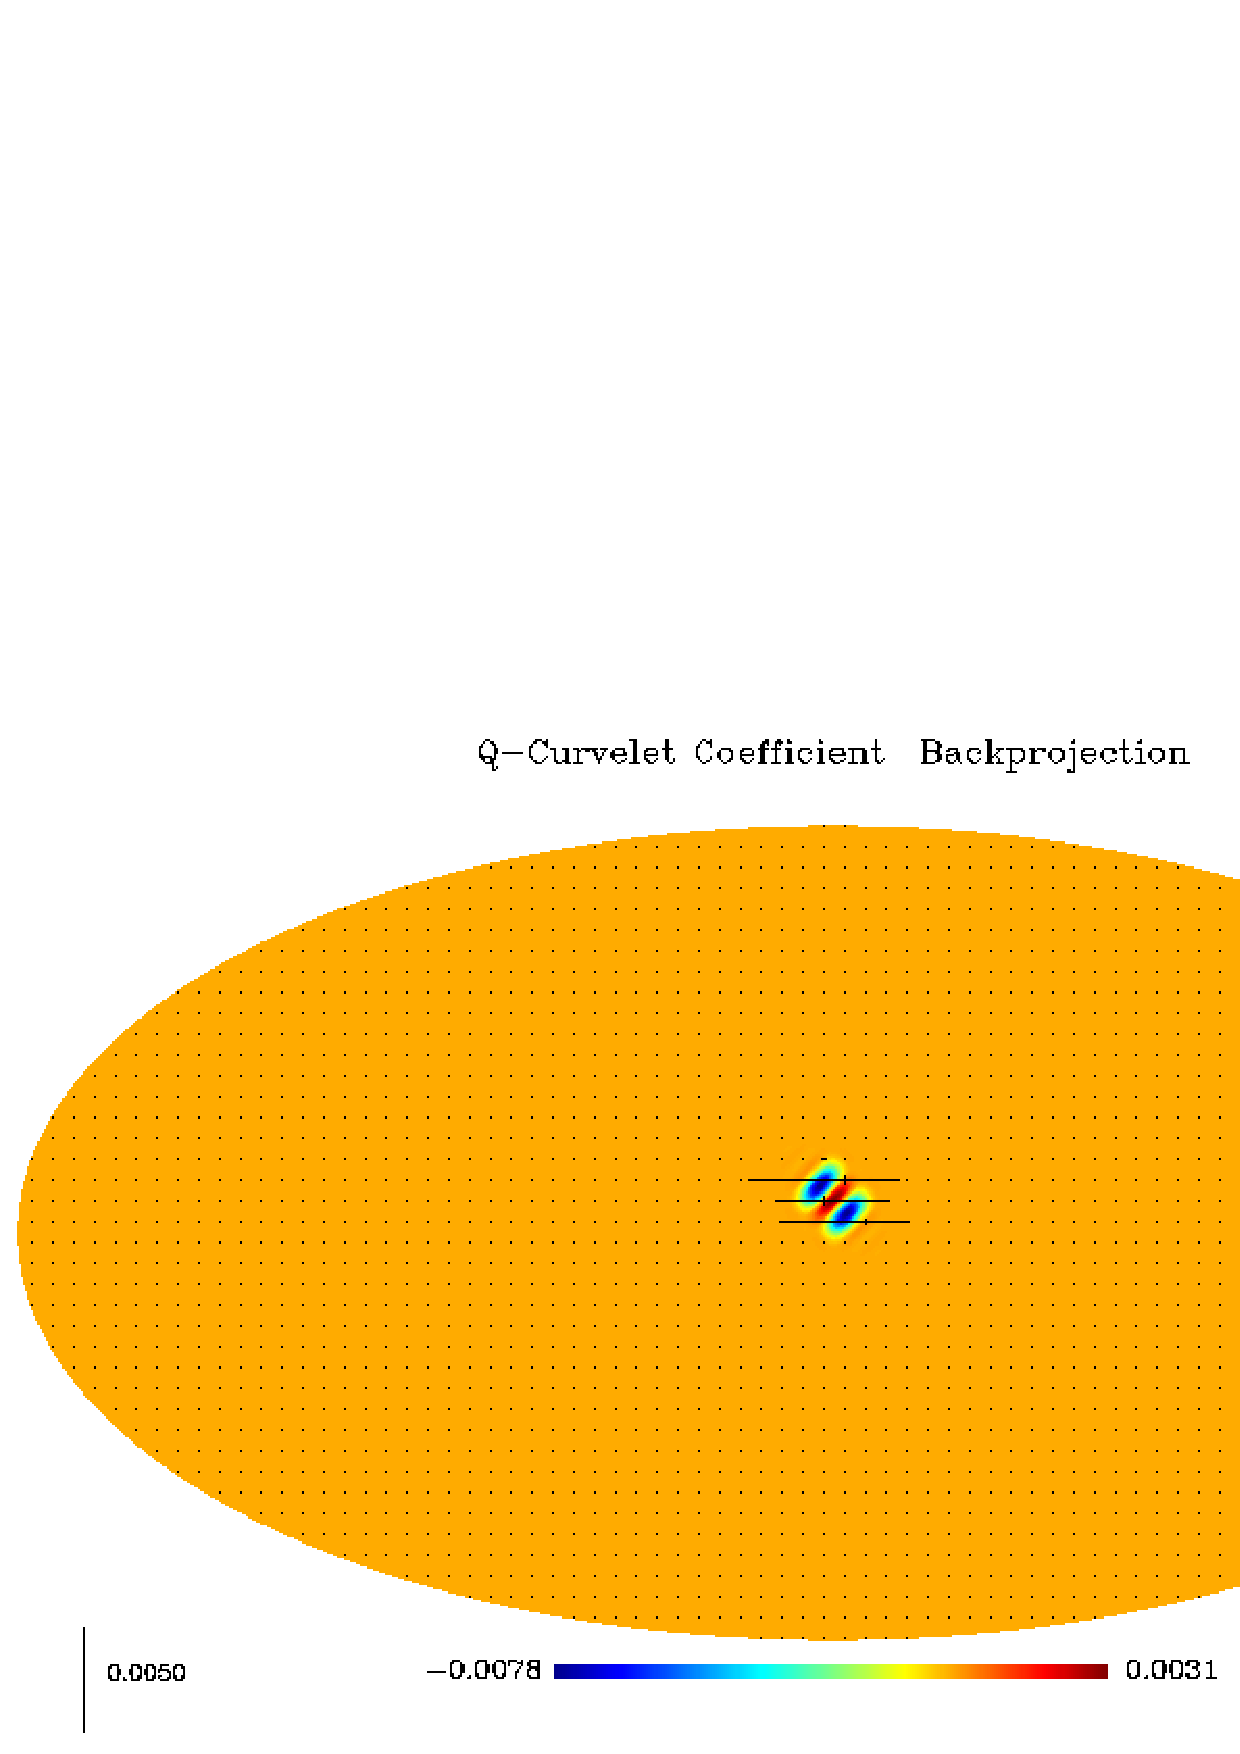
\includegraphics[width=7cm]{fig_mol_backproj_qucur_qj3.pdf}
 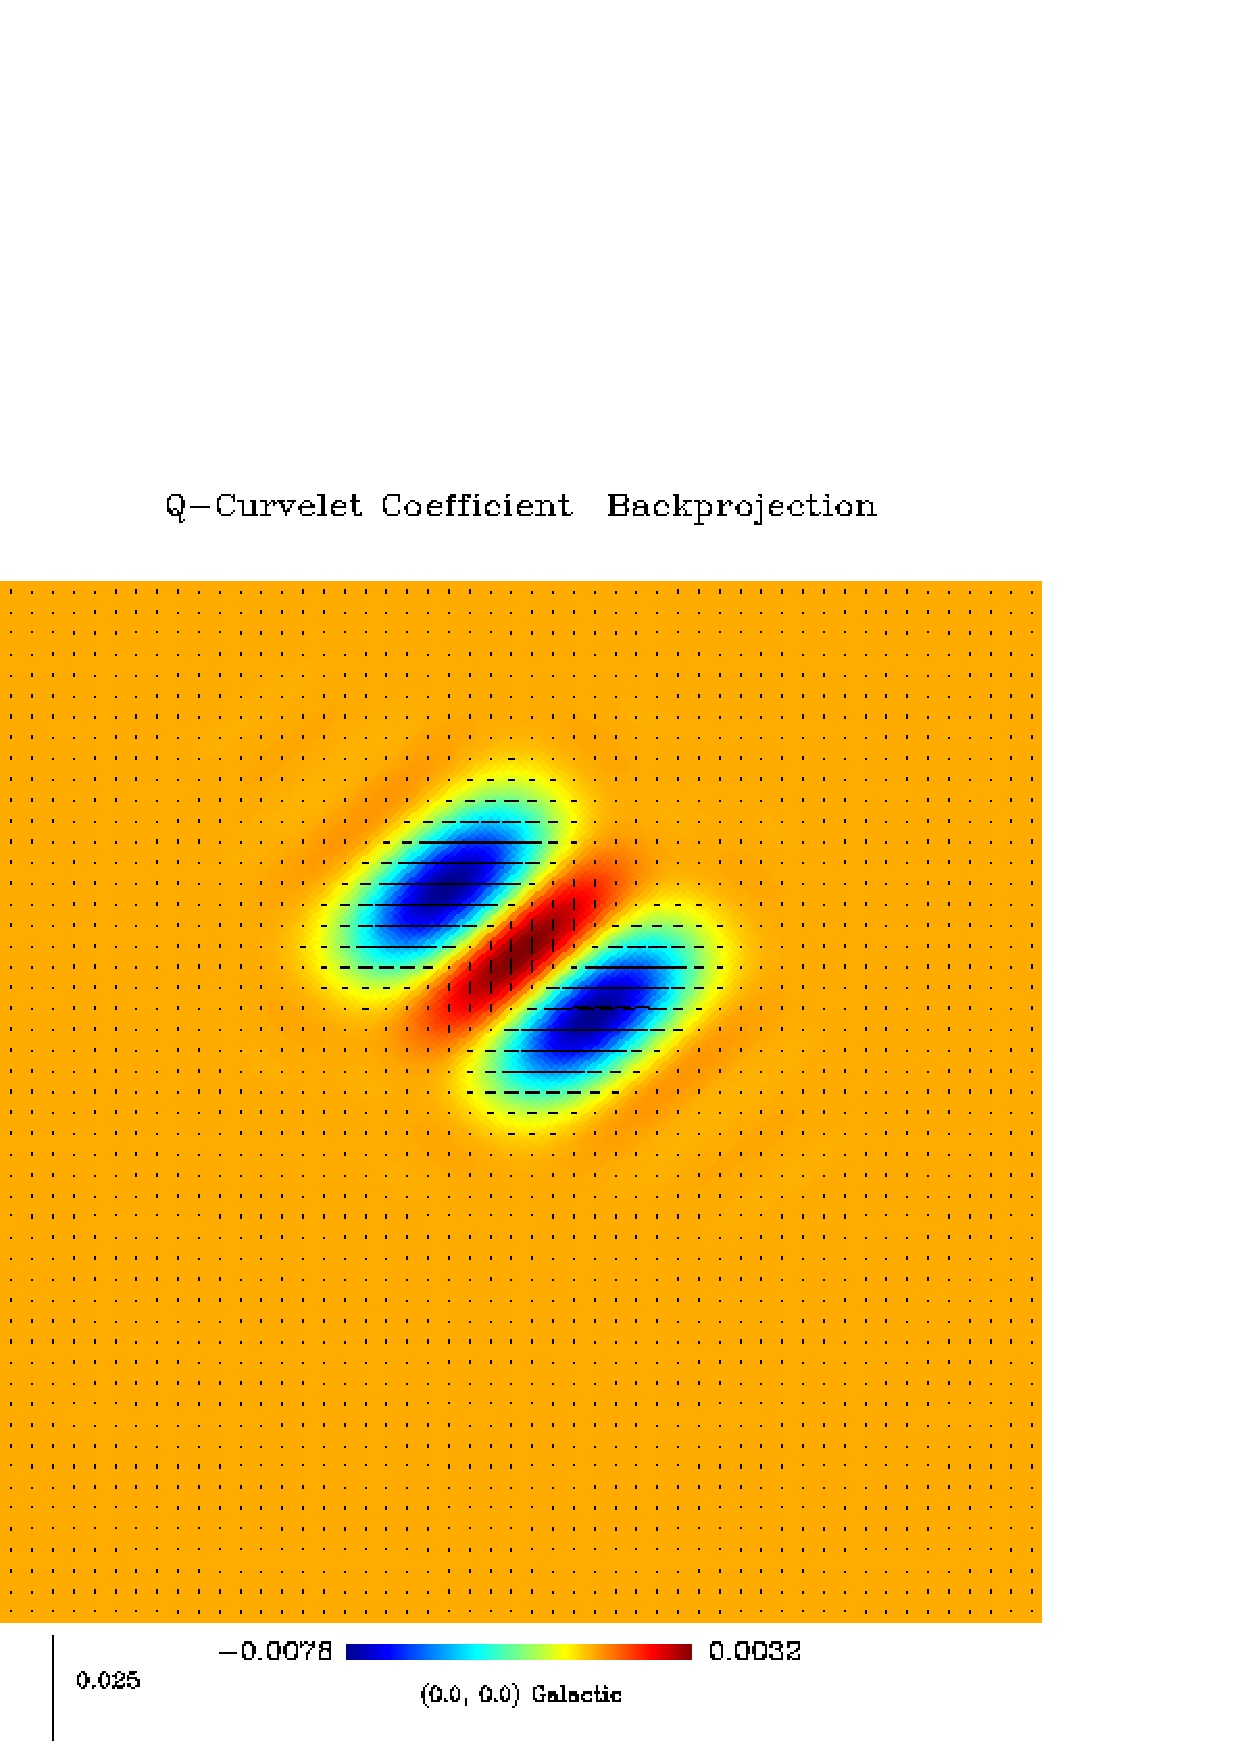
\includegraphics[width=4cm]{fig_backproj_qucur_qj3.pdf}
 }
 \hbox{
 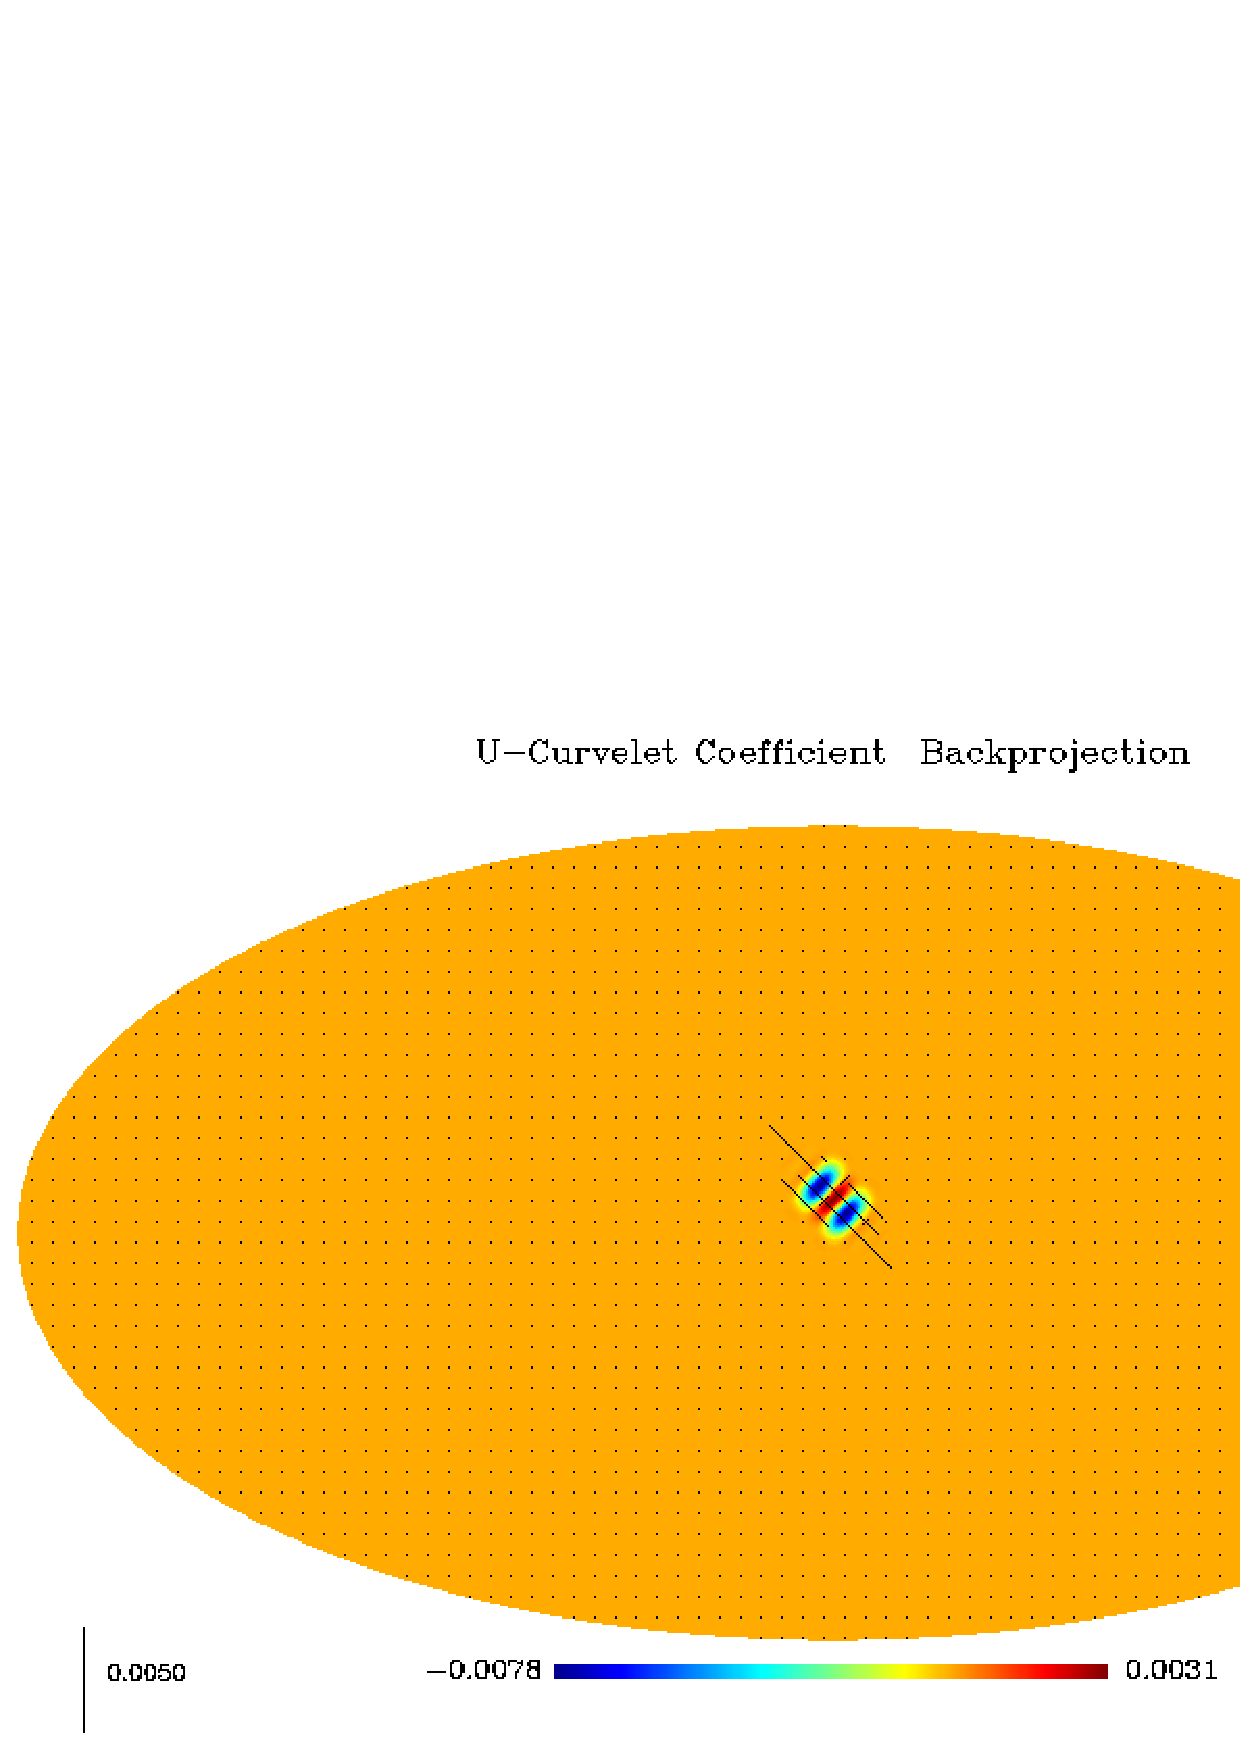
\includegraphics[width=7cm]{fig_mol_backproj_qucur_uj3.pdf}
 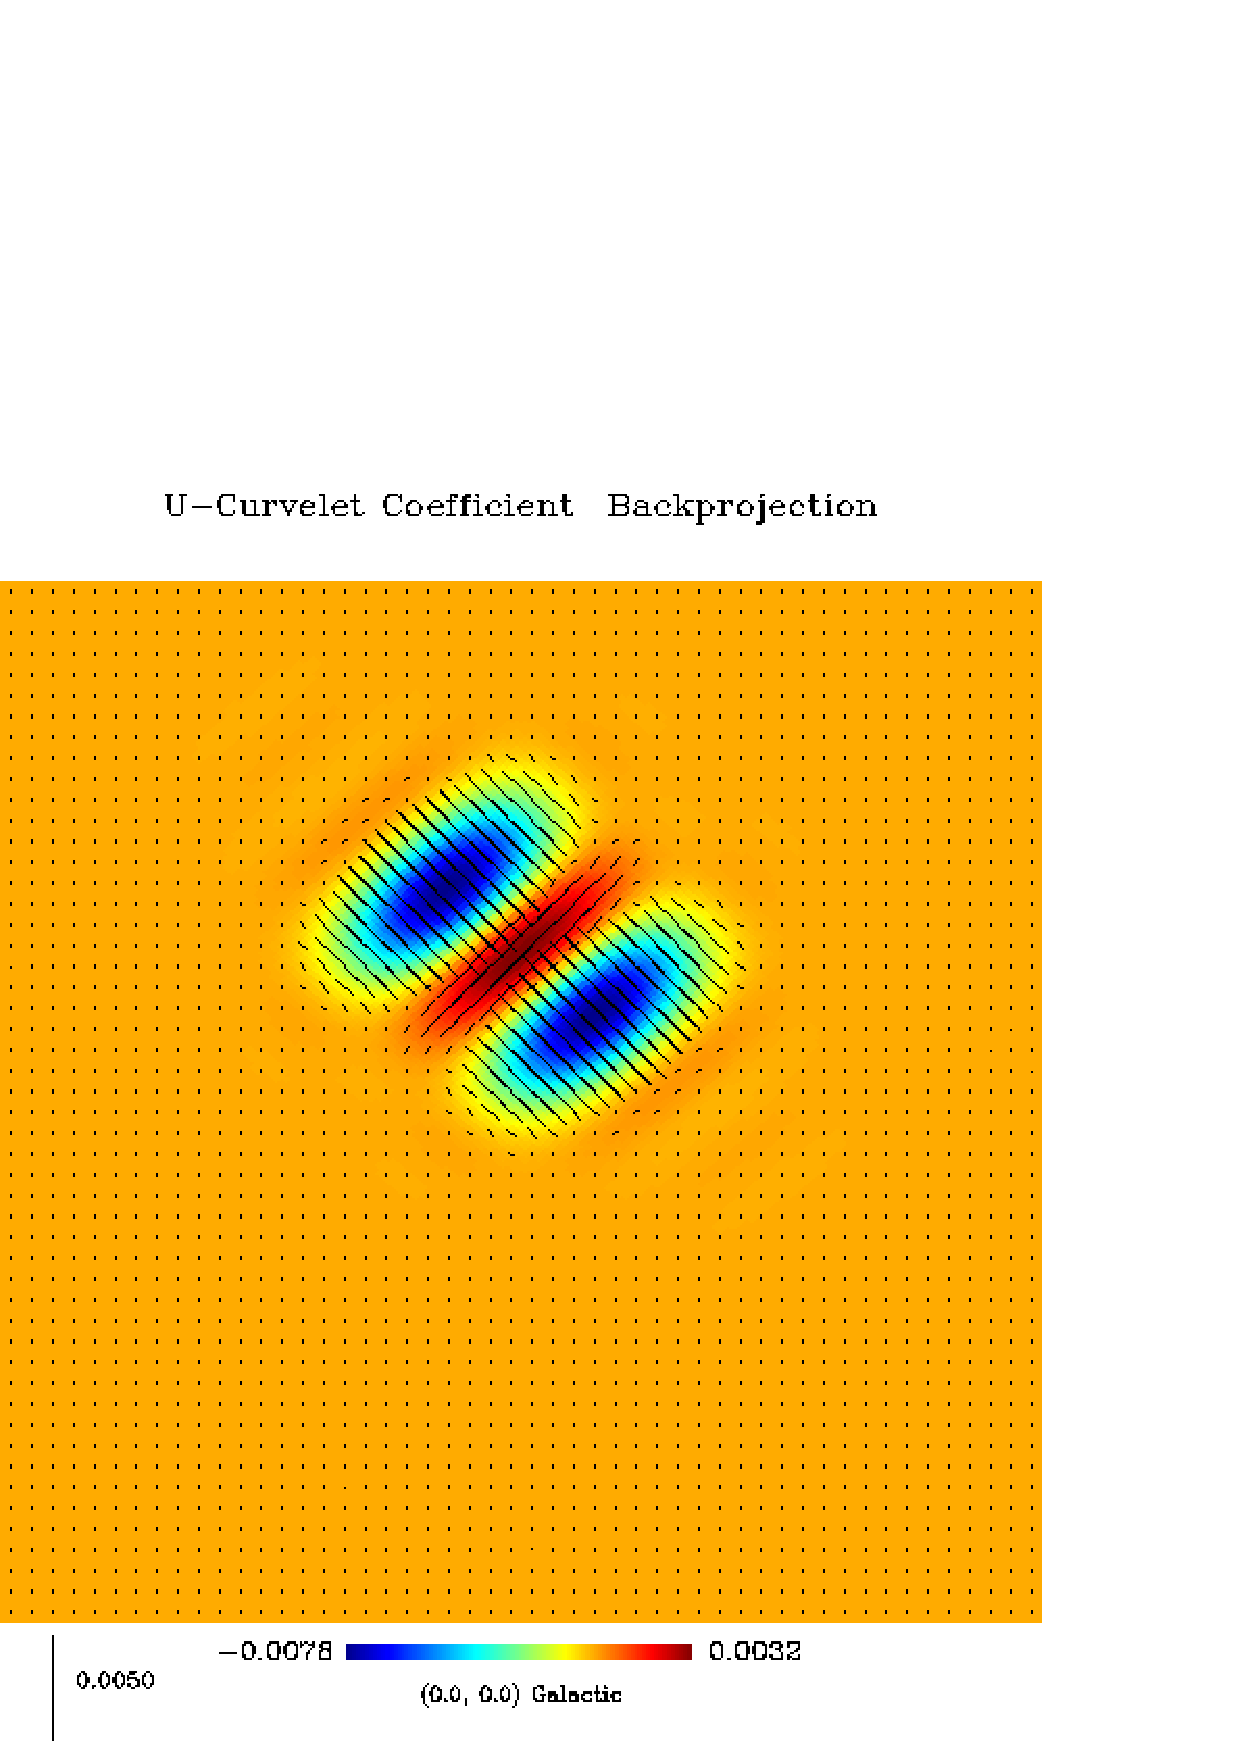
\includegraphics[width=4cm]{fig_backproj_qucur_uj3.pdf}
 }
  }
 }
\caption{Top, Q-curvelet backprojection (left)  and zoom (right). Bottom, U-curvelet backprojection (left)  and zoom. }
\label{fig_qucur_back}
\end{figure*}
The 2D ridgelet transform \cite{cur:candes99_1} was developed in an attempt to overcome some limitations inherent in former multiscale methods 
\emph{e.g.} the 2D wavelet, when handling smooth images with edges \textit{i.e.} singularities along smooth curves. Ridgelets are translation 
invariant \emph{ridge} functions with a wavelet profile in the normal direction. Although ridgelets provide sparse representations of smooth 
images with straight edges, they fail to efficiently handle edges along curved lines. This is the framework for curvelets which were given a 
first mathematical description in \cite{Curvelets-StMalo}. Basically, the curvelet dictionary is a multiscale pyramid of localized directional 
functions with anisotropic support obeying a specific parabolic scaling such that at scale $2^{-j}$, its length is $2^{-j/2}$ and its width is $2^{-j}$. 
This is motivated by the parabolic scaling property of smooth curves. Other properties of the curvelet transform as well as decisive optimality results 
in approximation theory are reported in \cite{Curvelets-StMalo,CandesDonohoCurvelets}. Notably, curvelets provide optimally sparse representations 
of manifolds which are smooth away from edge singularities along smooth curves. Several digital curvelet transforms \cite{cur:donoho99,starck:sta01_3,cur:demanet06} 
have been proposed which attempt to preserve the essential properties of the continuous curvelet transform and many papers \cite{starck:sta04,felix2008,starck:sta04} 
report on their successful application in image processing experiments. The so-called first generation discrete curvelet described in \cite{cur:donoho99,starck:sta01_3} 
consists in applying the ridgelet transform to sub-images of a wavelet decomposition of the original image. By construction, the sub-images are 
well localized in space and frequency and the subsequent ridgelet transform provides the necessary directional sensitivity. This latter implementation 
in combination with the good geometric properties of the Healpix pixelization scheme, inspired the digital curvelet transform on the sphere~\cite{starck:sta05_2}. 
The digital curvelet transform on the sphere is clearly invertible in the sense that each step of the overall transform is itself invertible. 
The curvelet transform on the sphere has a redundancy factor of $16J + 1$ when $J$ scales are used, which may be a problem for handling huge data sets 
such as from the future Planck-Surveyor experiment. This can be reduced by substituting the pyramidal wavelet transform to the undecimated wavelet 
transform in the above algorithm. More details on the wavelet, ridgelet, curvelet algorithms on the sphere can be found in \cite{starck:sta05_2}. 
As for the isotropic wavelet on the sphere, a straightforward extension to polarized data will consist in applying successively the curvelet transform 
on the sphere to the three components $T$, $Q$ and $U$. Figure~\ref{fig_qucur_back} shows the backprojection of a Q-curvelet coefficient and 
U-curvelet coefficient. Clearly, the shapes of these polarized curvelet functions are very different from the polarized wavelet functions.%---------------------------------------------------------------------------------------------------------------------------------------
%---------------------------------------------------------------------------------------------------------------------------------------
\section{Polarized E/B Wavelet and E/B Curvelet}
\label{sec:pol_eb}

\subsection{Introduction}
We have seen that the generalization of the Fourier representation for polarized data on the sphere is the spin-2 spherical harmonics basis denoted $_{\pm 2}Y_{\ell m}$: 
\begin{equation} 
Q \pm i U  = \sum_{\ell, m}  { _{\pm 2}a_{\ell m}}   {_{\pm 2}Y_{\ell m} }
\end{equation} 
  
At this point, it is convenient~\cite{zalda} to introduce the two quantities denoted $E$ and $B$ which are defined on the sphere by 
\begin{eqnarray}\label{EB}
E = &  \sum_{\ell, m}   a_{\ell m} ^E Y_{\ell m} =  \sum_{\ell, m}  - \frac{ 1}{2}   ({_{ 2}a_{\ell m}}  +  {_{- 2}a_{\ell m}} )    Y_{\ell m} \\ \nonumber
B = & \sum_{\ell, m}   a_{\ell m} ^B Y_{\ell m} =  \sum_{\ell, m}  i \frac{ 1}{2}    ({_{ 2}a_{\ell m}}  -  {_{- 2}a_{\ell m}} )   Y_{\ell m} 
\end{eqnarray} 
%\begin{equation}\label{EB}
%E =  \sum_{\ell, m}   a_{\ell m} ^E Y_{\ell m} =  \sum_{\ell, m}  - \frac{   {_{ 2}a_{\ell m}}  +  {_{- 2}a_{\ell m}}  }  {2}  Y_{\ell m}  \quad \quad 
%B =  \sum_{\ell, m}   a_{\ell m} ^B Y_{\ell m} =  \sum_{\ell, m}  i \frac{   {_{ 2}a_{\ell m}}  -  {_{- 2}a_{\ell m}}  }  {2}   Y_{\ell m} 
%\end{equation} 
where $Y_{\ell m}$ stands for the usual spin 0 spherical harmonics basis functions. The quantities $E$ and $B$ are derived by applying 
the spin lowering operator twice to $Q + i U$  and the spin raising operator twice to $Q - i U$ so that $E$ and $B$ are real scalar 
fields on the sphere, invariant through rotations of the local reference frame. The normalization of $a_{\ell m} ^E$ and $a_{\ell m} ^B$ 
chosen in the latter definition is purely conventional but it appears to be rather popular~\cite{1997PhRvD..55.1830Z,2003PhRvD..67b3501B}. 
Still, we could multiply $a_{\ell m} ^E$ and $a_{\ell m} ^B$ by some $A_{\ell}$ and we would have just as good a representation of the initial 
polarization maps. Through a change of parity $E$ will remain invariant whereas the sign of pseudo-scalar $B$ will change. The $E$ and $B$ 
modes defined here are not so different from the \emph{gradient} (\emph{i.e. curl} free) and \emph{curl} (\emph{i.e. divergence} free) components 
encountered in the analysis of vector fields. Finally, the spatial anisotropies of the Gaussian CMB temperature and polarization fields are 
completely characterized in this new linear representation by the power spectra and cross spectra of $T$, $E$ and $B$. Thanks to the different 
parities of $T$ and $E$ on one side and $B$ on the other, the sufficient statistics reduce to only four spectra namely $C_\ell^{EE}, C_\ell^{TE}, 
C_\ell^{TT}, C_\ell^{BB}$. For a given cosmological model, it is possible to give a theoretical prediction of these spectra. Aiming at inverting 
the model and inferring the cosmological parameters, an important goal of CMB temperature and polarization data analysis is then to estimate the 
latter power spectra, based on sampled, noisy sometimes incomplete $T$, $Q$ and $U$ spherical maps.  

\subsection{E/B Isotropic Wavelet}
Following the above idea of representing CMB polarization maps by means of $E$ and $B$ modes, we propose a formal extension of the previous 
undecimated isotropic wavelet transform that will allow us to handle linear polarization data maps $T$, $Q$ and $U$ on the sphere. Practically, 
the maps we consider are pixelized using for instance the Healpix pixelization scheme. In fact, we are not concerned at this point with the 
recovery of E and B modes from pixelized or incomplete data maps which itself is not a trivial task. The extension of the wavelet transform 
on the sphere we describe here makes use of the $E$ and $B$ representation of polarized maps described above in a formal way. Given polarization 
data maps $T$, $Q$ and $U$, the proposed wavelet transform algorithm consists of the following steps : 
\vspace{.1cm}
\begin{center}
\begin{minipage}[b]{0.85\linewidth}
\footnotesize{
\begin{enumerate}
\item Apply the spin $\pm 2$ spherical harmonics transform to $Q+iU$ and $Q-iU$. Practically, the Healpix software package provides an implementation 
of this transform for maps that use this pixelization scheme. Otherwise, a fast implementation was recently proposed by \cite{wiauxspin2}.
\item Combine the decomposition coefficients ${ _{2}a_{\ell m}}$ and ${ _{-2}a_{\ell m}}$ from the first step into $a_{\ell m}^E$ and $a_{\ell m}^B$ 
and build \emph{formal} $E$ and $B$ maps associated with $Q$ and $U$ by applying the usual inverse spherical harmonics transform, as in equation~\ref{EB}. 
For numerical and algorithmic purposes, it may be efficient to stay with the spherical harmonics representation of $E$ and $B$.
\item Apply the undecimated isotropic transform on the sphere described above to map $T$ and to the $E$, $B$ representation of the polarization maps. 
\end{enumerate}}
\end{minipage}
\end{center}
\vspace{.1cm}
The wavelet coefficient maps  $w_j^T$, $w_j^E$, $w_j^B$ and the low resolution approximation maps $c_J^T$, $c_J^E$, $c_J^B$ are obtained by applying 
the isotropic undecimated wavelet transform described in section~\ref{sec:UWTS} to the $T$, $E$, $B$ representation of the polarized data. Figure~\ref{fig:UWTSpol} 
shows the result of applying the proposed transform to the polarized CMB data map \emph{ka} \footnote{available at http://lambda.gsfc.nasa.gov/product/map/current/ } 
from the WMAP experiment. The top two images show the initial $Q$ and $U$ maps while the subsequent maps are the low pass and wavelet coefficients'maps 
in a four scale decomposition. The scaling function we used is a cubic box spline as proposed in section~\ref{sec:UWTS}. The wavelet coefficients were 
obtained as the difference between two successive low pass approximations of the multiresolution decomposition of the $E$ and $B$ maps. The proper choice 
for the scaling and wavelet functions will depend on the application and the existence of constraints to be enforced.
\begin{figure*}
\vbox{
\centerline{
\hbox{
\psfig{figure=ka_q_nb_hi.pdf,bbllx=5cm,bblly=2cm,bburx= 19cm,bbury=28cm,height=7cm,width=4cm,angle = 90,clip=}
\psfig{figure=ka_u_nb_hi.pdf,bbllx=5cm,bblly=2cm,bburx= 19cm,bbury=28cm,height=7cm,width=4cm,angle = 90,clip=}
}
}
\centerline{
\hbox{
\psfig{figure=ka__hi3_1_nb.pdf,bbllx=5cm,bblly=2cm,bburx= 19cm,bbury=28cm,height=7cm,width=4cm,angle = 90,clip=}
\psfig{figure=ka__hi3_2_nb.pdf,bbllx=5cm,bblly=2cm,bburx= 19cm,bbury=28cm,height=7cm,width=4cm,angle = 90,clip=}
}
}
\centerline{
\hbox{
\psfig{figure=ka__hi2_1_nb.pdf,bbllx=5cm,bblly=2cm,bburx= 19cm,bbury=28cm,height=7cm,width=4cm,angle = 90,clip=}
\psfig{figure=ka__hi2_2_nb.pdf,bbllx=5cm,bblly=2cm,bburx= 19cm,bbury=28cm,height=7cm,width=4cm,angle = 90,clip=}
}
}
\centerline{
\hbox{
\psfig{figure=ka__hi1_1_nb.pdf,bbllx=5cm,bblly=2cm,bburx= 19cm,bbury=28cm,height=7cm,width=4cm,angle = 90,clip=}
\psfig{figure=ka__hi1_2_nb.pdf,bbllx=5cm,bblly=2cm,bburx= 19cm,bbury=28cm,height=7cm,width=4cm,angle = 90,clip=}
}
}
\centerline{
\hbox{
\psfig{figure=ka__hi0_1_nb.pdf,bbllx=5cm,bblly=2cm,bburx= 19cm,bbury=28cm,height=7cm,width=4cm,angle = 90,clip=}
\psfig{figure=ka__hi0_2_nb.pdf,bbllx=5cm,bblly=2cm,bburx= 19cm,bbury=28cm,height=7cm,width=4cm,angle = 90,clip=}
}
}
}
\caption{\textbf{top~:} $Q$ and $U$ CMB polarization data maps from channel \emph{ka} of the WMAP experiment. \textbf{left~:} low pass and wavelet coefficients in three scales of the formal E mode. \textbf{right~:} low pass and wavelet coefficients in three scales of the formal B mode.}
\label{fig:UWTSpol}
\end{figure*}

%---------------------------------------------------------------------------------------------------------------------------------------
\subsection*{Reconstruction}
%---------------------------------------------------------------------------------------------------------------------------------------
\begin{figure*}[htb]
\centerline{
\vbox{
 \hbox{
 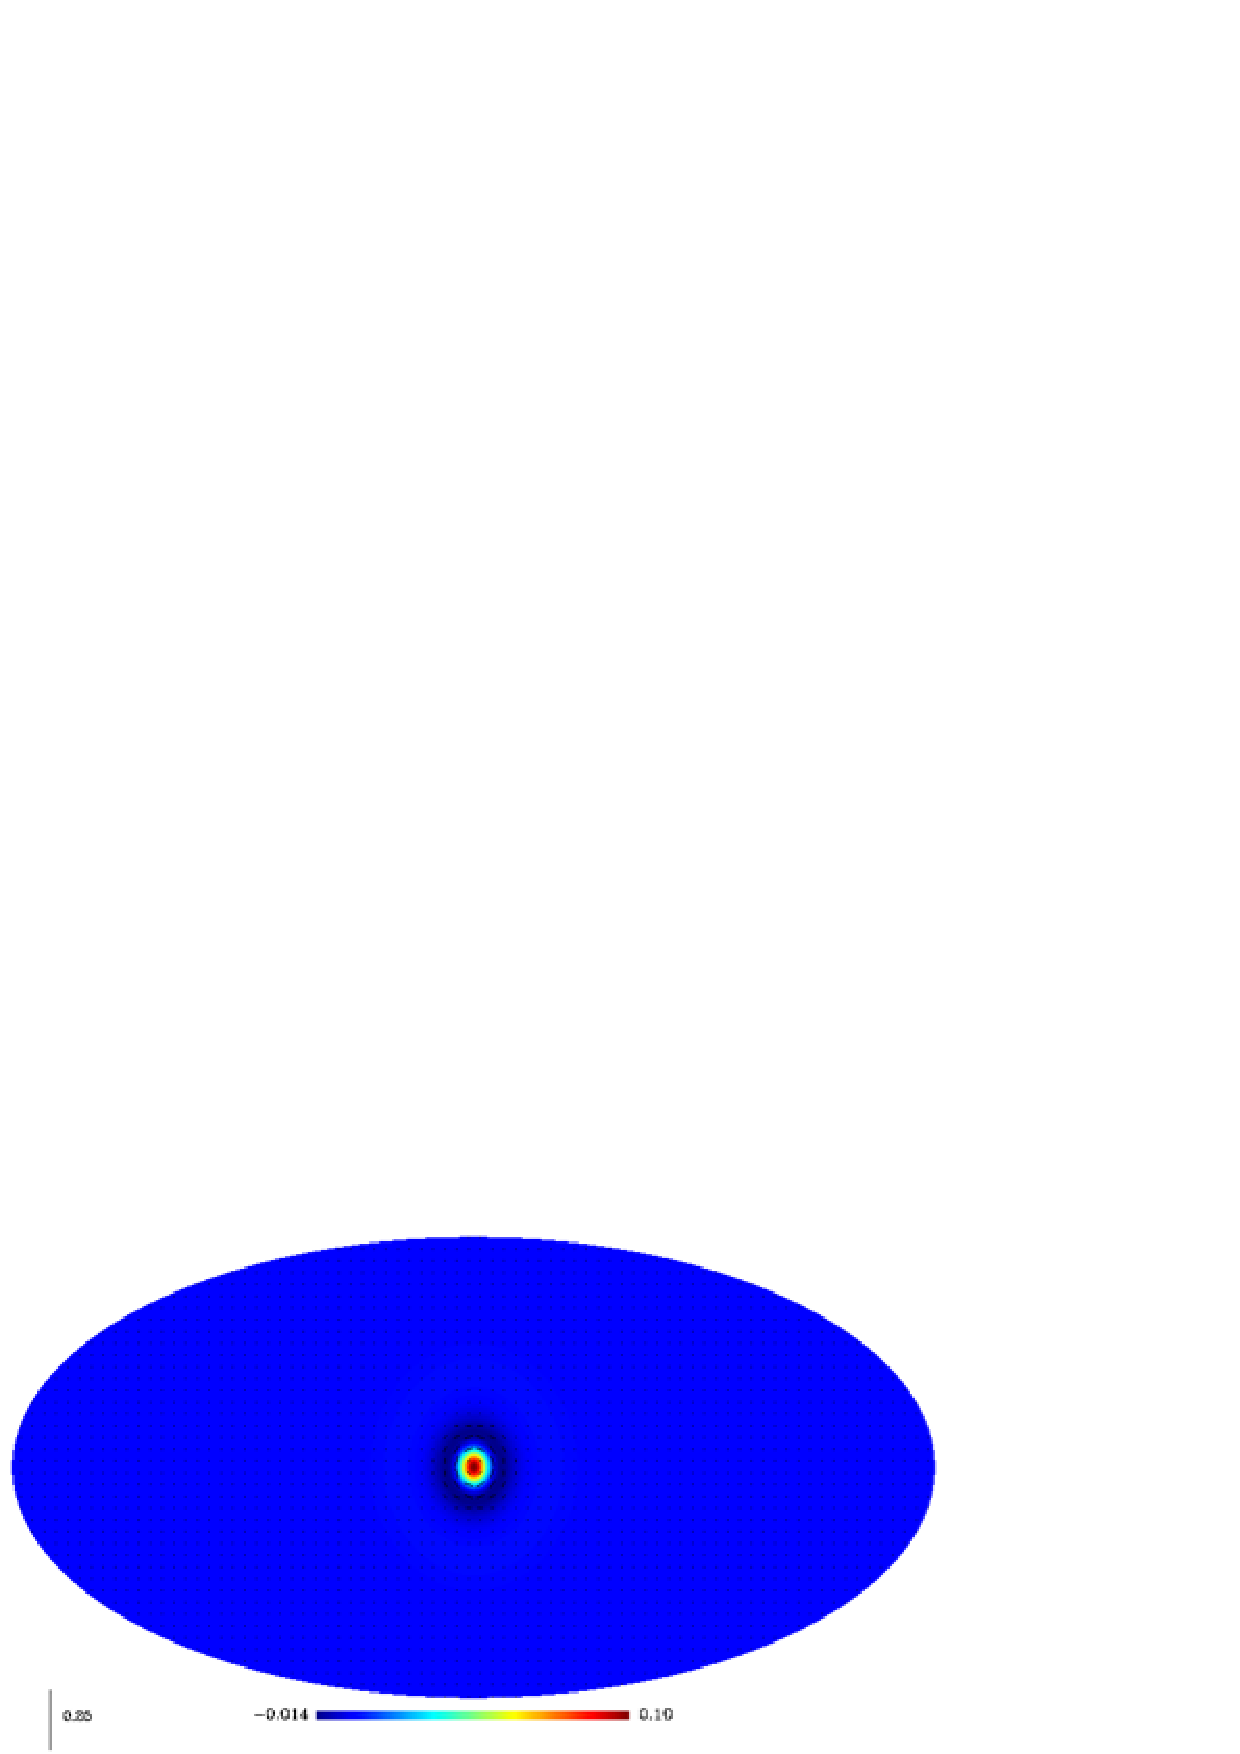
\includegraphics[width=7cm]{fig_e_iwt_back_scale2.pdf}
 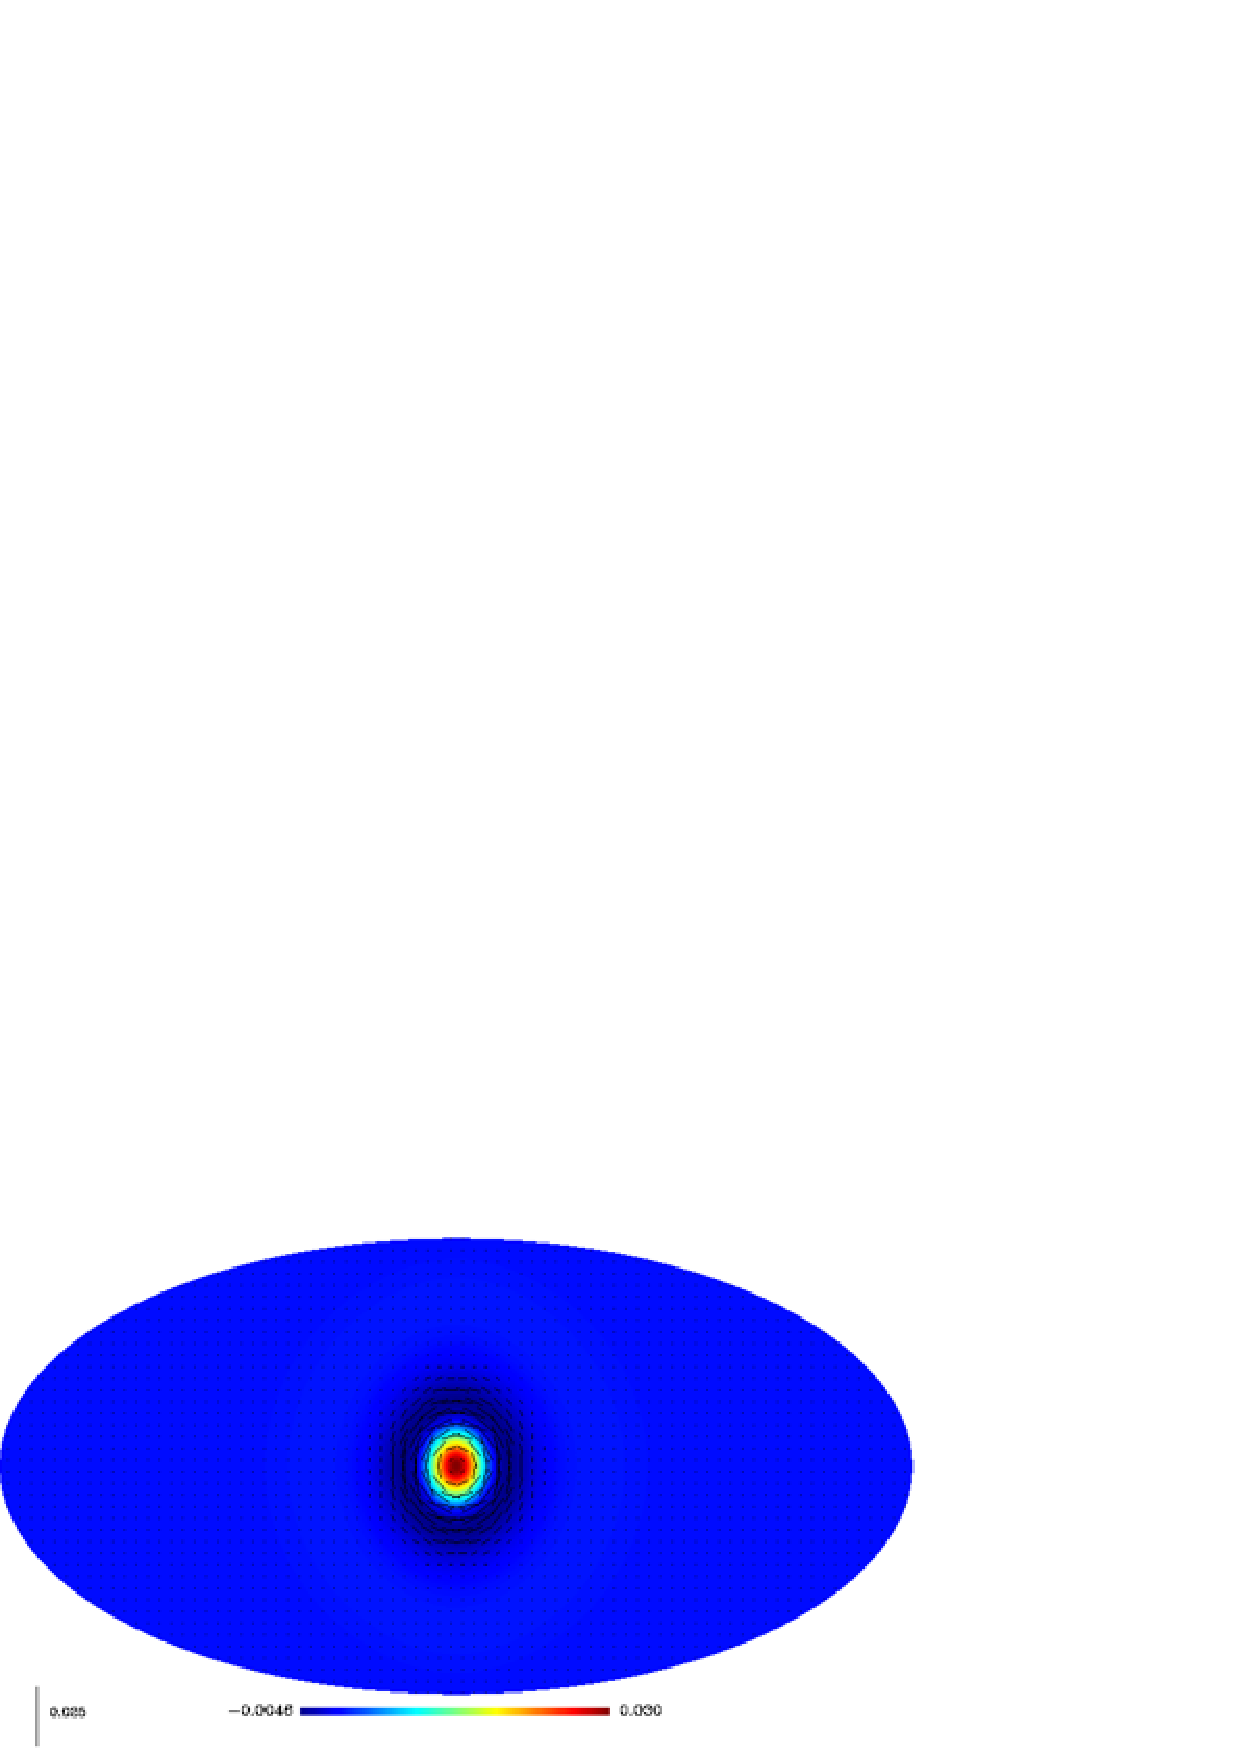
\includegraphics[width=7cm]{fig_b_iwt_back_scale2.pdf}
 }
  \hbox{
 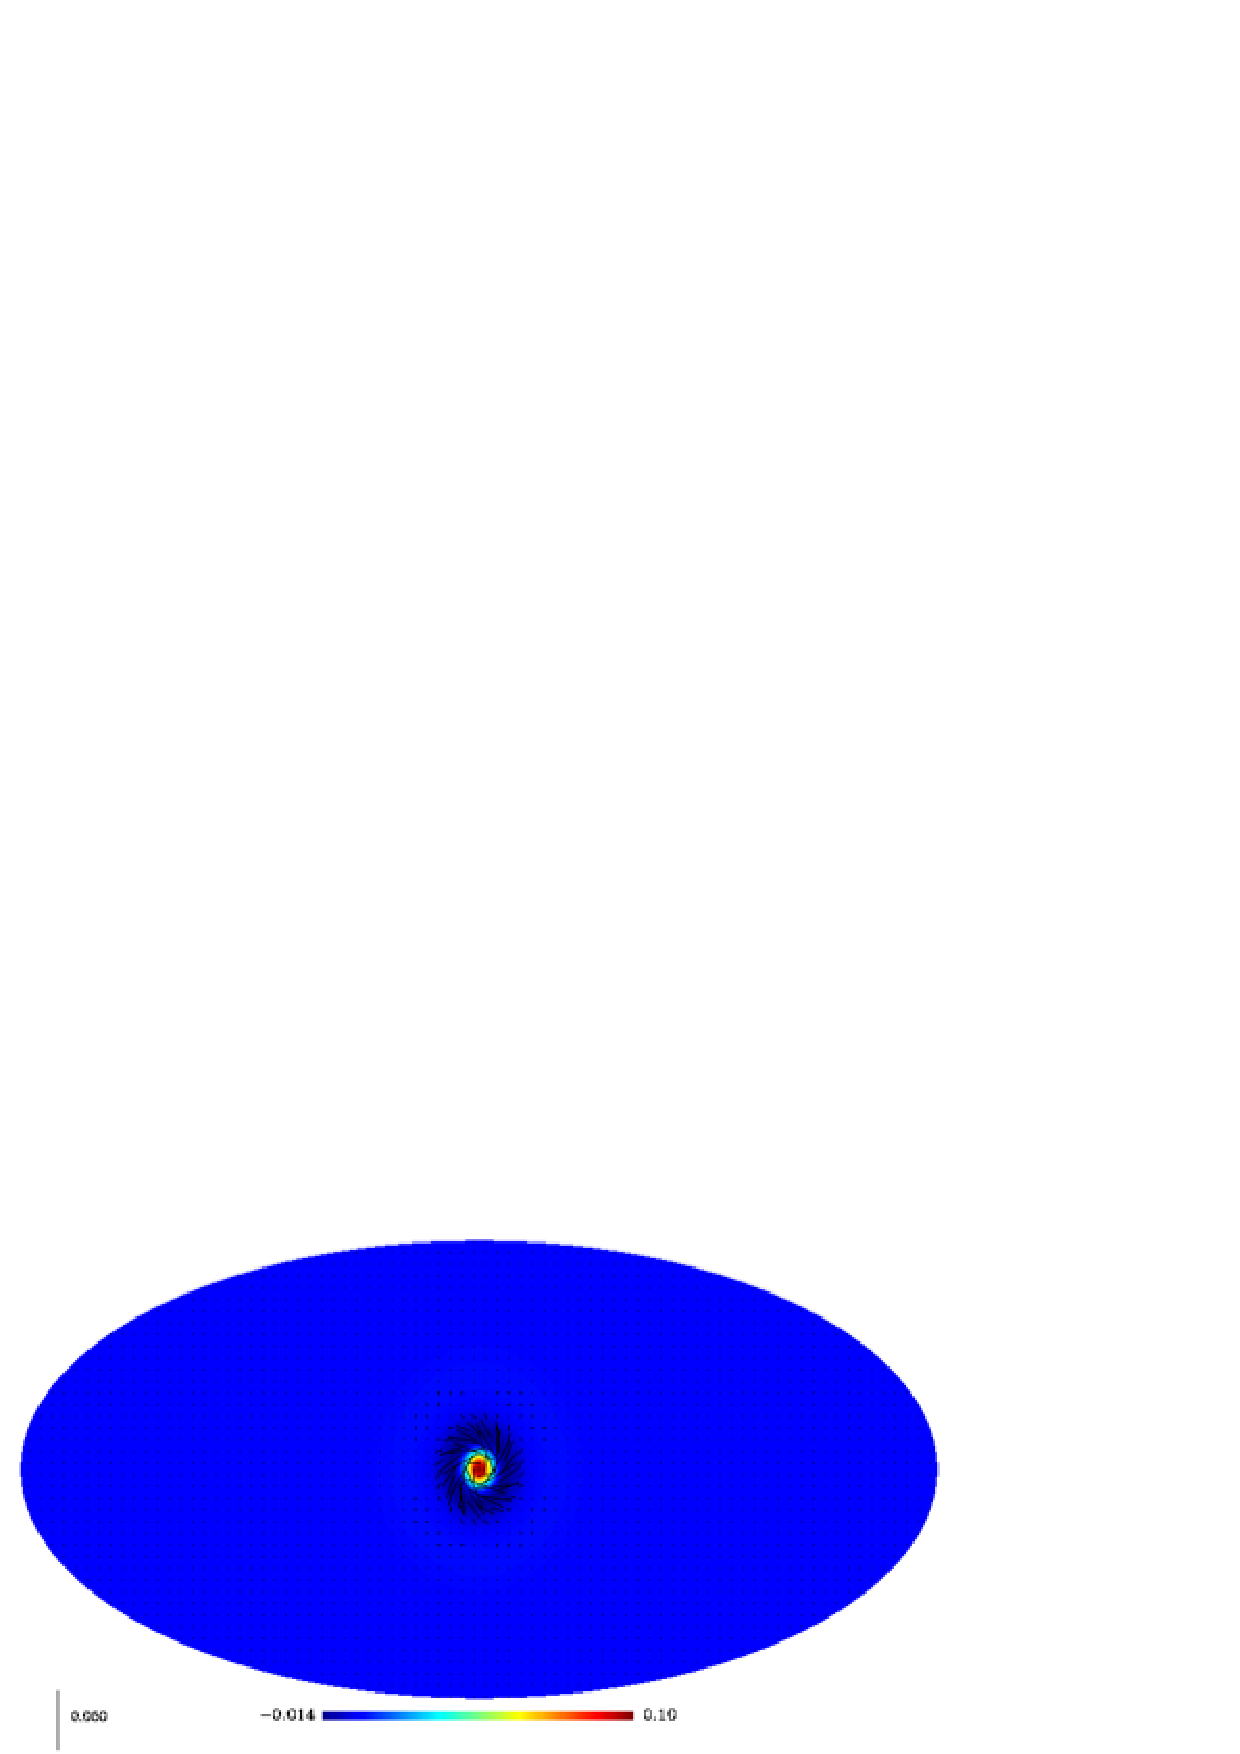
\includegraphics[width=7cm]{fig_e_iwt_back_scale3.pdf}
 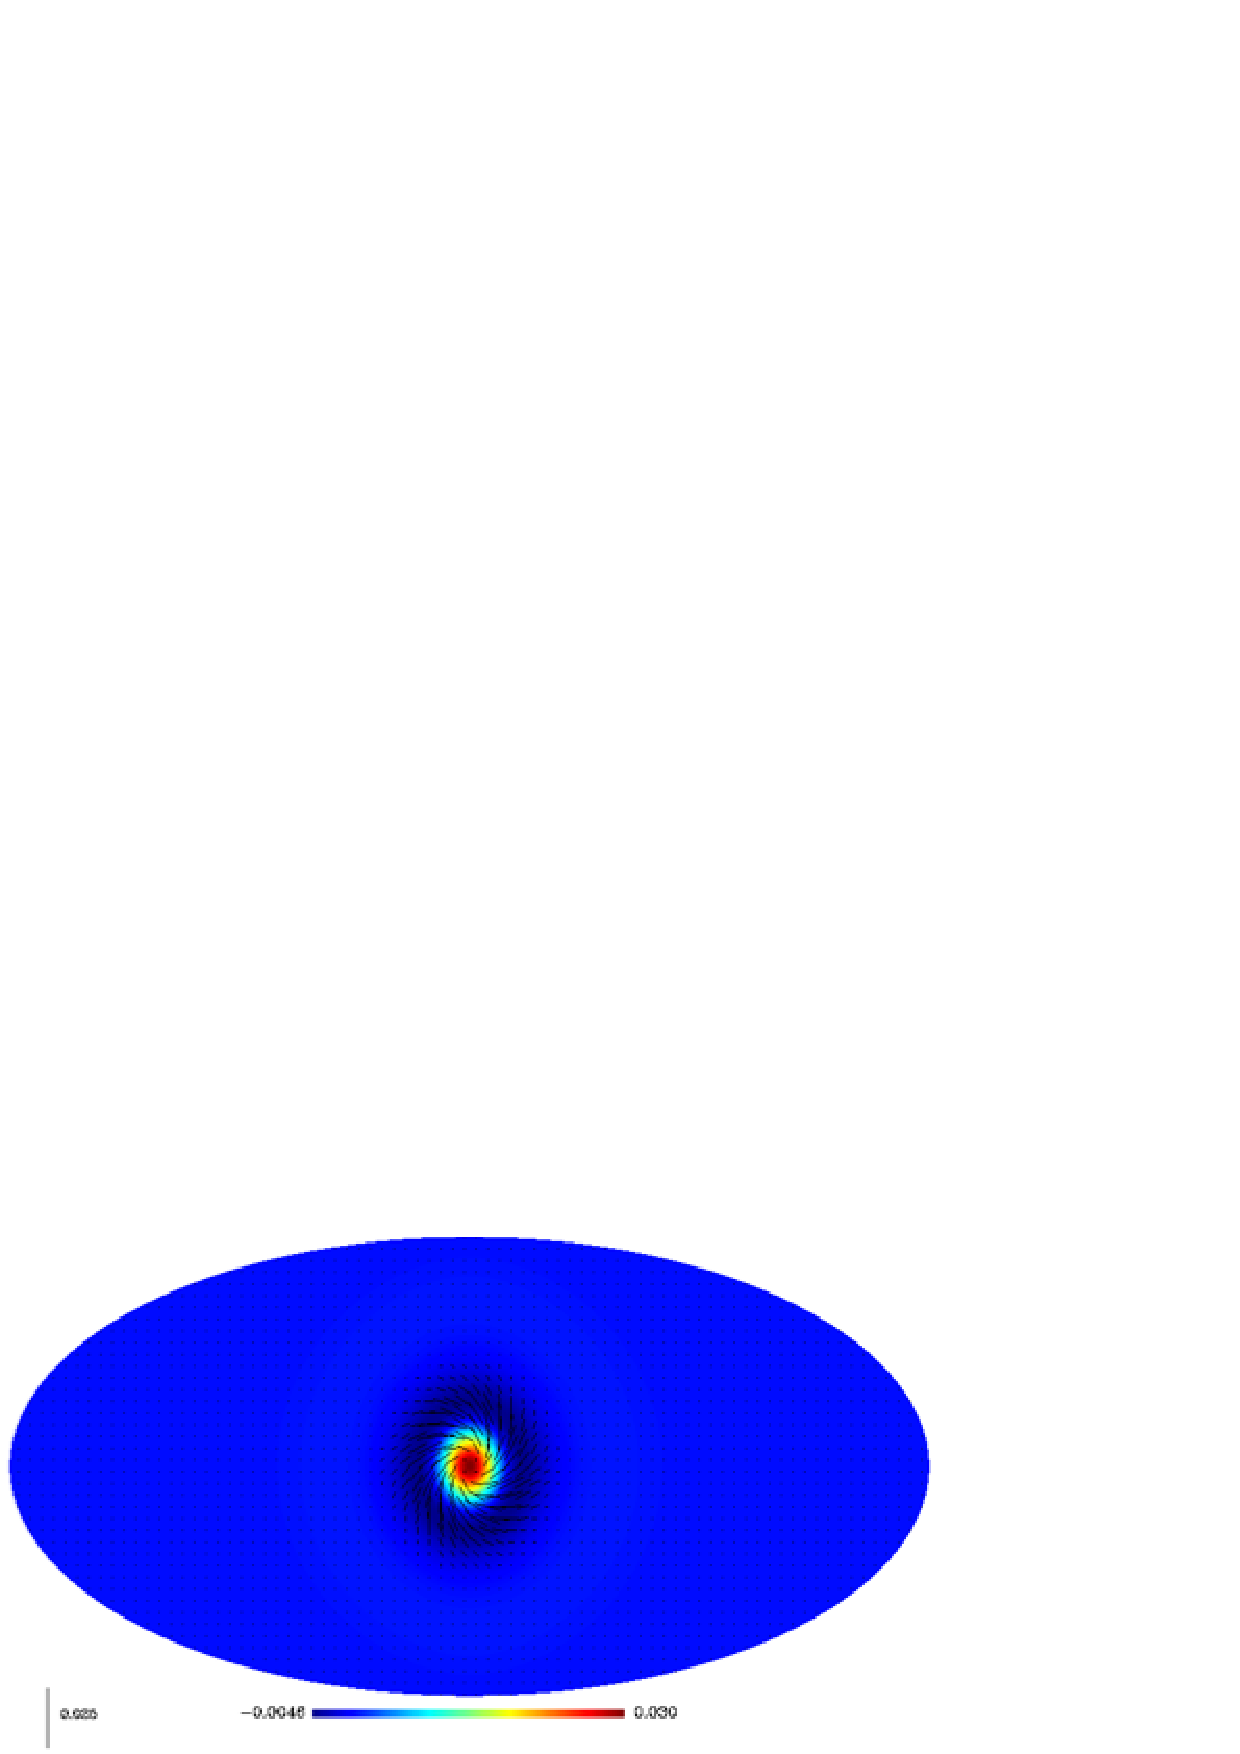
\includegraphics[width=7cm]{fig_b_iwt_back_scale3.pdf}
 }
 \hbox{
 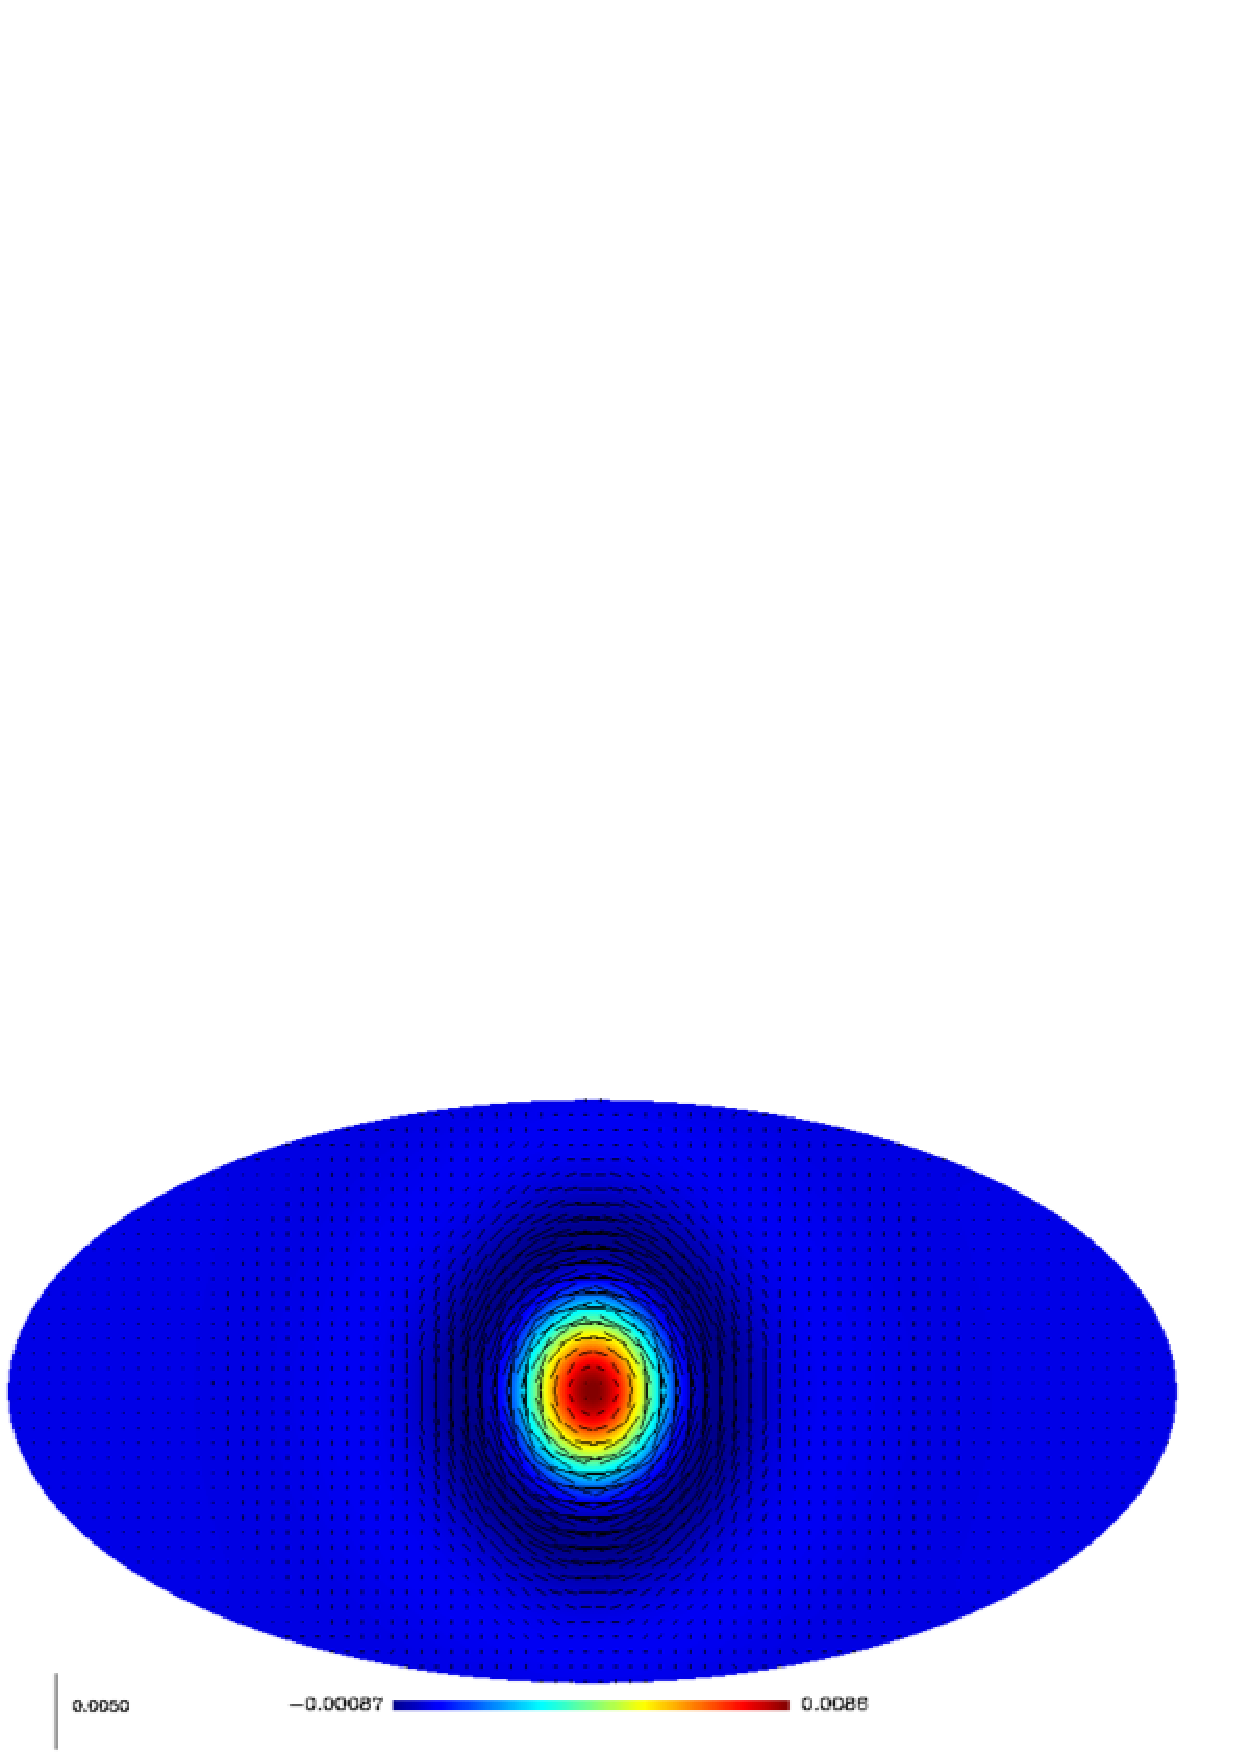
\includegraphics[width=7cm]{fig_e_iwt_back_scale4.pdf}
 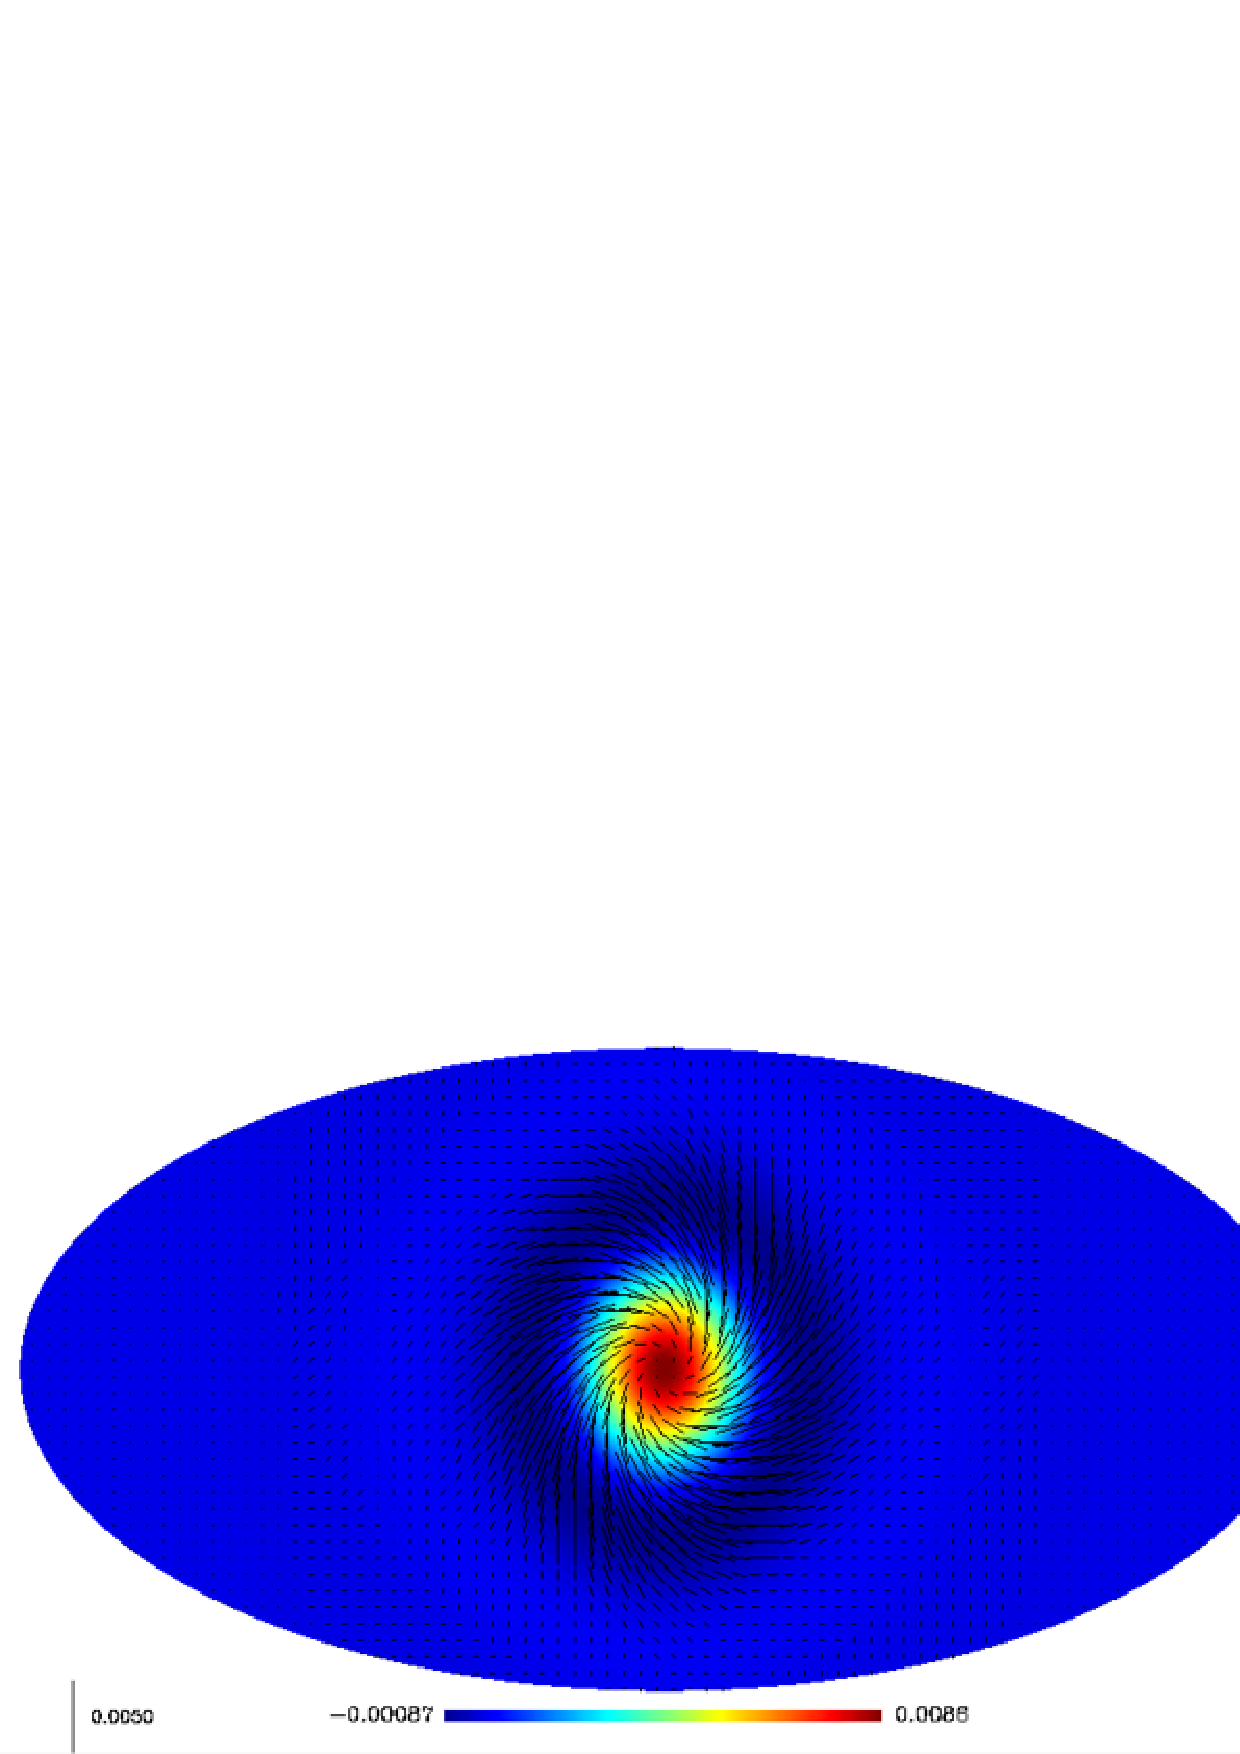
\includegraphics[width=7cm]{fig_b_iwt_back_scale4.pdf}
 }
 }
 }
\caption{E-isotropic wavelet transform backprojection (left) and B-isotropic wavelet backprojection (right).}
\label{fig_eb_iwt_back}
\end{figure*}
Obviously, the transform described above is invertible and the inverse transform is readily obtained by applying the inverse 
of each of the three steps in reverse order. If, as in the example decomposition above, we take the wavelet function to be 
the difference between two successive low pass approximations, the third step is inverted by simply summing the last low pass 
approximation with the maps of wavelet coefficients from all scales as in equation~\ref{IWT} : 
\begin{eqnarray}
T  & = & c_{J}^T + \sum_{j=1}^{J} w_j^T \quad \quad \nonumber \\
E & = & c_{J}^E + \sum_{j=1}^{J} w_j^E \quad \quad \nonumber \\
B & = &  c_{J}^B + \sum_{j=1}^{J} w_j^B
\end{eqnarray}
where $c_{J}^X$ stands for the low resolution approximation to component $X$ and $w_j^X$ is the map of wavelet coefficients of that component on scale $j$. Finally, noting that : 
\begin{eqnarray}
Q  & =  & -\frac{1}{2} \sum_{\ell, m}   a_{\ell m} ^E   ( {_{ 2} Y}_{\ell m} +  {_{ -2} Y}_{\ell m} ) +  i a_{\ell m} ^B ( {_{ 2} Y}_{\ell m} -  {_{ -2} Y}_{\ell m} )  \nonumber \\
     & =  & \sum_{\ell, m}   a_{\ell m} ^E   Z_{\ell m}^+ +  i a_{\ell m} ^B Z_{\ell m}^-   \\ \nonumber
U  & =   & -\frac{1}{2} \sum_{\ell, m}   a_{\ell m} ^B   ( {_{ 2} Y}_{\ell m} +  {_{ -2} Y}_{\ell m} ) -  i a_{\ell m} ^E ( {_{ 2} Y}_{\ell m} -  {_{ -2} Y}_{\ell m} )  \nonumber \\
      & =  & \sum_{\ell, m}   a_{\ell m} ^B Z_{\ell m}^+ -  i a_{\ell m} ^E Z_{\ell m}^-   
\end{eqnarray}
the initial representation of the polarized data in terms of $T$, $Q$ and $U$ maps is reconstructed from its wavelet coefficients using the following equations : 
% \begin{eqnarray}
%T= c_{J}^T + \sum_{j=1}^{J} w_j^T \\ \nonumber
%Q = \Big \{ \sum_{\ell, m}   <  c_{J}^E , Y_{\ell m}>  {_{ +} Z}_{\ell m} +  i <  c_{J}^B , Y_{\ell m}>  {_{ -} Z}_{\ell m} \Big \}        +   \sum_{j=1}^{J}  \Big \{ \sum_{\ell, m}  <  w_j^E , Y_{\ell m}>  {_{ +} Z}_{\ell m} +  i <  w_j^B , Y_{\ell m}>  {_{ -} Z}_{\ell m} \Big \}    \\ \nonumber 
%U = \Big \{ \sum_{\ell, m}   <  c_{J}^B , Y_{\ell m}>  {_{ +} Z}_{\ell m}  -  i <  c_{J}^E , Y_{\ell m}>  {_{ -} Z}_{\ell m} \Big \}        +   \sum_{j=1}^{J}  \Big \{ \sum_{\ell, m}  <  w_j^B , Y_{\ell m}>  {_{ +} Z}_{\ell m} -  i <  w_j^E , Y_{\ell m}>  {_{ -} Z}_{\ell m} \Big \}    
%\end{eqnarray}
%\begin{eqnarray}
%T =& c_{J}^T + \sum_{j=1}^{J} w_j^T \\ \nonumber
%Q =& c_{J}^E  \sum_{\ell, m} Y_{\ell m}^{\dagger} Z_{\ell m}^+ + i c_{J}^B  \sum_{\ell, m} Y_{\ell m} ^{\dagger} Z_{\ell m}^-  +   \sum_{j=1}^{J}  \Big \{  w_j^E  \sum_{\ell, m} Y_{\ell m}^{\dagger} Z_{\ell m}^+ +{i} w_j^B  \sum_{\ell, m} Y_{\ell m}^{\dagger}  Z_{\ell m}^- \Big \}    \\ \nonumber 
%U =& c_{J}^B  \sum_{\ell, m} Y_{\ell m}^{\dagger} Z_{\ell m}^+ -  i c_{J}^E  \sum_{\ell, m} Y_{\ell m} ^{\dagger} Z_{\ell m}^-  +   \sum_{j=1}^{J}  \Big \{  w_j^B  \sum_{\ell, m} Y_{\ell m}^{\dagger} Z_{\ell m}^+ - {i} w_j^E  \sum_{\ell, m} Y_{\ell m}^{\dagger}  Z_{\ell m}^- \Big \}   
%\end{eqnarray}
\begin{eqnarray}\label{eq:recons}
T =& c_{J}^T + \sum_{j=1}^{J} w_j^T \\ \nonumber
Q =& c_{J}^{E,+} + i c_{J}^{B,-} + \sum_{j=1}^{J} \Big \{ w_j^{E,+} + i w_j^{B,-} \Big \} \\ \nonumber 
U =& c_{J}^{B,+} - i c_{J}^{E,-} + \sum_{j=1}^{J} \Big \{ w_j^{B,+} - i w_j^{E,-} \Big \}
\end{eqnarray}
where
\begin{eqnarray}\label{eq:change}
c_{J}^{X,+} = c_{J}^X \sum_{\ell, m} Y_{\ell m}^{\dagger} Z_{\ell m}^+ \quad \textrm{and} \quad c_{J}^{X,-} = c_{J}^X \sum_{\ell, m} Y_{\ell m}^{\dagger} Z_{\ell m}^- 
\end{eqnarray}
with $W^\dagger$ denoting the transpose conjugate of $W$ so that $\tilde{W} W^\dagger$ is the scalar dot product of $\tilde{W}$ and $W$ 
while $W^\dagger \tilde{W}$ is an operator (or matrix) acting on its left hand side as a projection along $W$ and \emph{reconstruction} 
along $\tilde{W}$. In practice, the Healpix software package provides us with an implementation of the forward and inverse spin $0$ and 
spin $2$ spherical harmonics transforms which we need to implement the proposed inverse transform given by equations~\ref{eq:recons} 
and~\ref{eq:change}. Clearly, as mentioned earlier in section~\ref{sec:UWTS}, we could have chosen some other wavelet function than merely 
the difference between two consecutive scaling functions, and the transformation would still be nearly as simple to invert. Fig.\ref{fig_eb_iwt_back} 
shows, on the left, backprojections of E-wavelet coefficients, and, on the right, backprojections of B-wavelet coefficients on the right hand side at different scales.

%---------------------------------------------------------------------------------------------------------------------------------------
\subsection*{E-B  Curvelet}
%---------------------------------------------------------------------------------------------------------------------------------------
\begin{figure*}[htb]
\centerline{
\vbox{
 \hbox{
 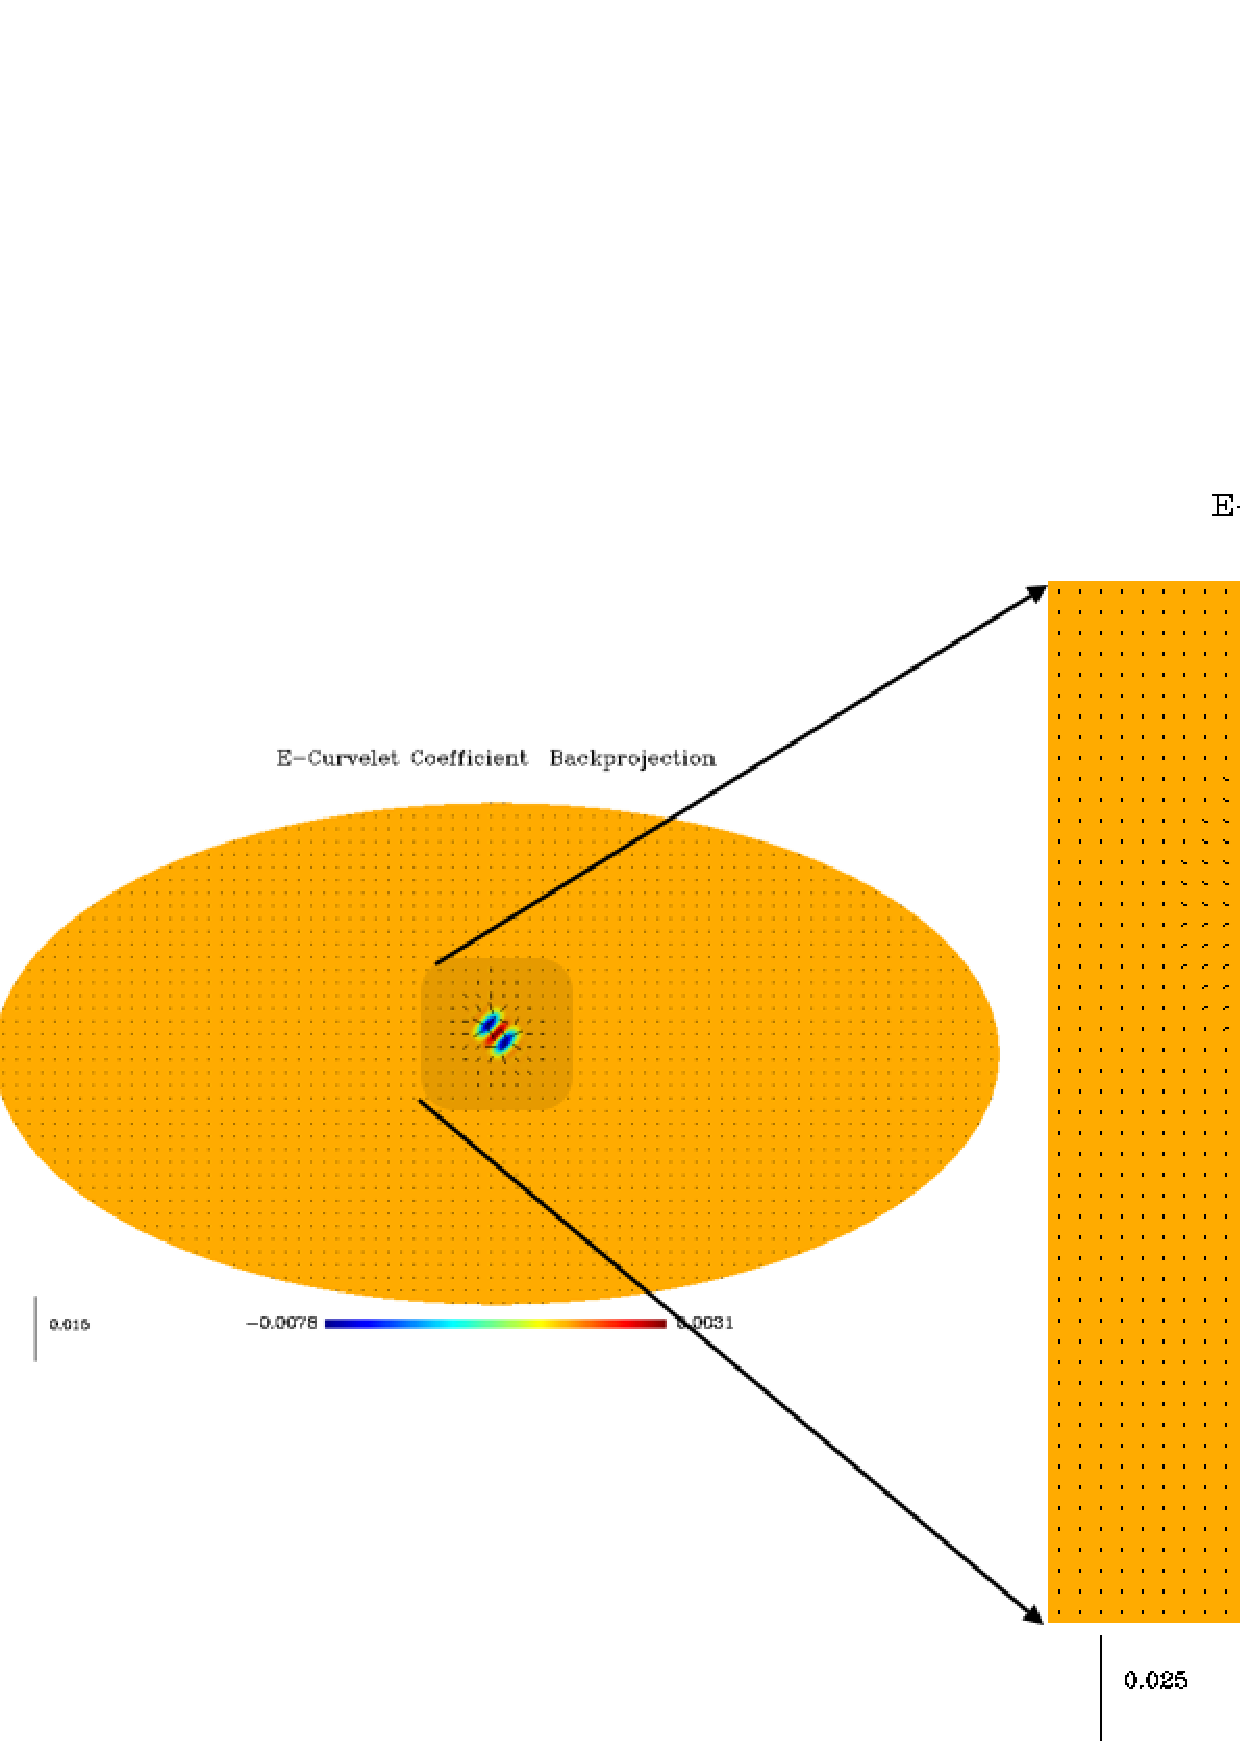
\includegraphics[width=12cm]{fig_ecur_back.pdf}
 }
  }
 }
\caption{E-curvelet coefficient backprojection.}
\label{fig_ecur_back}
\end{figure*}

\begin{figure*}[htb]
\centerline{
\vbox{
 \hbox{
 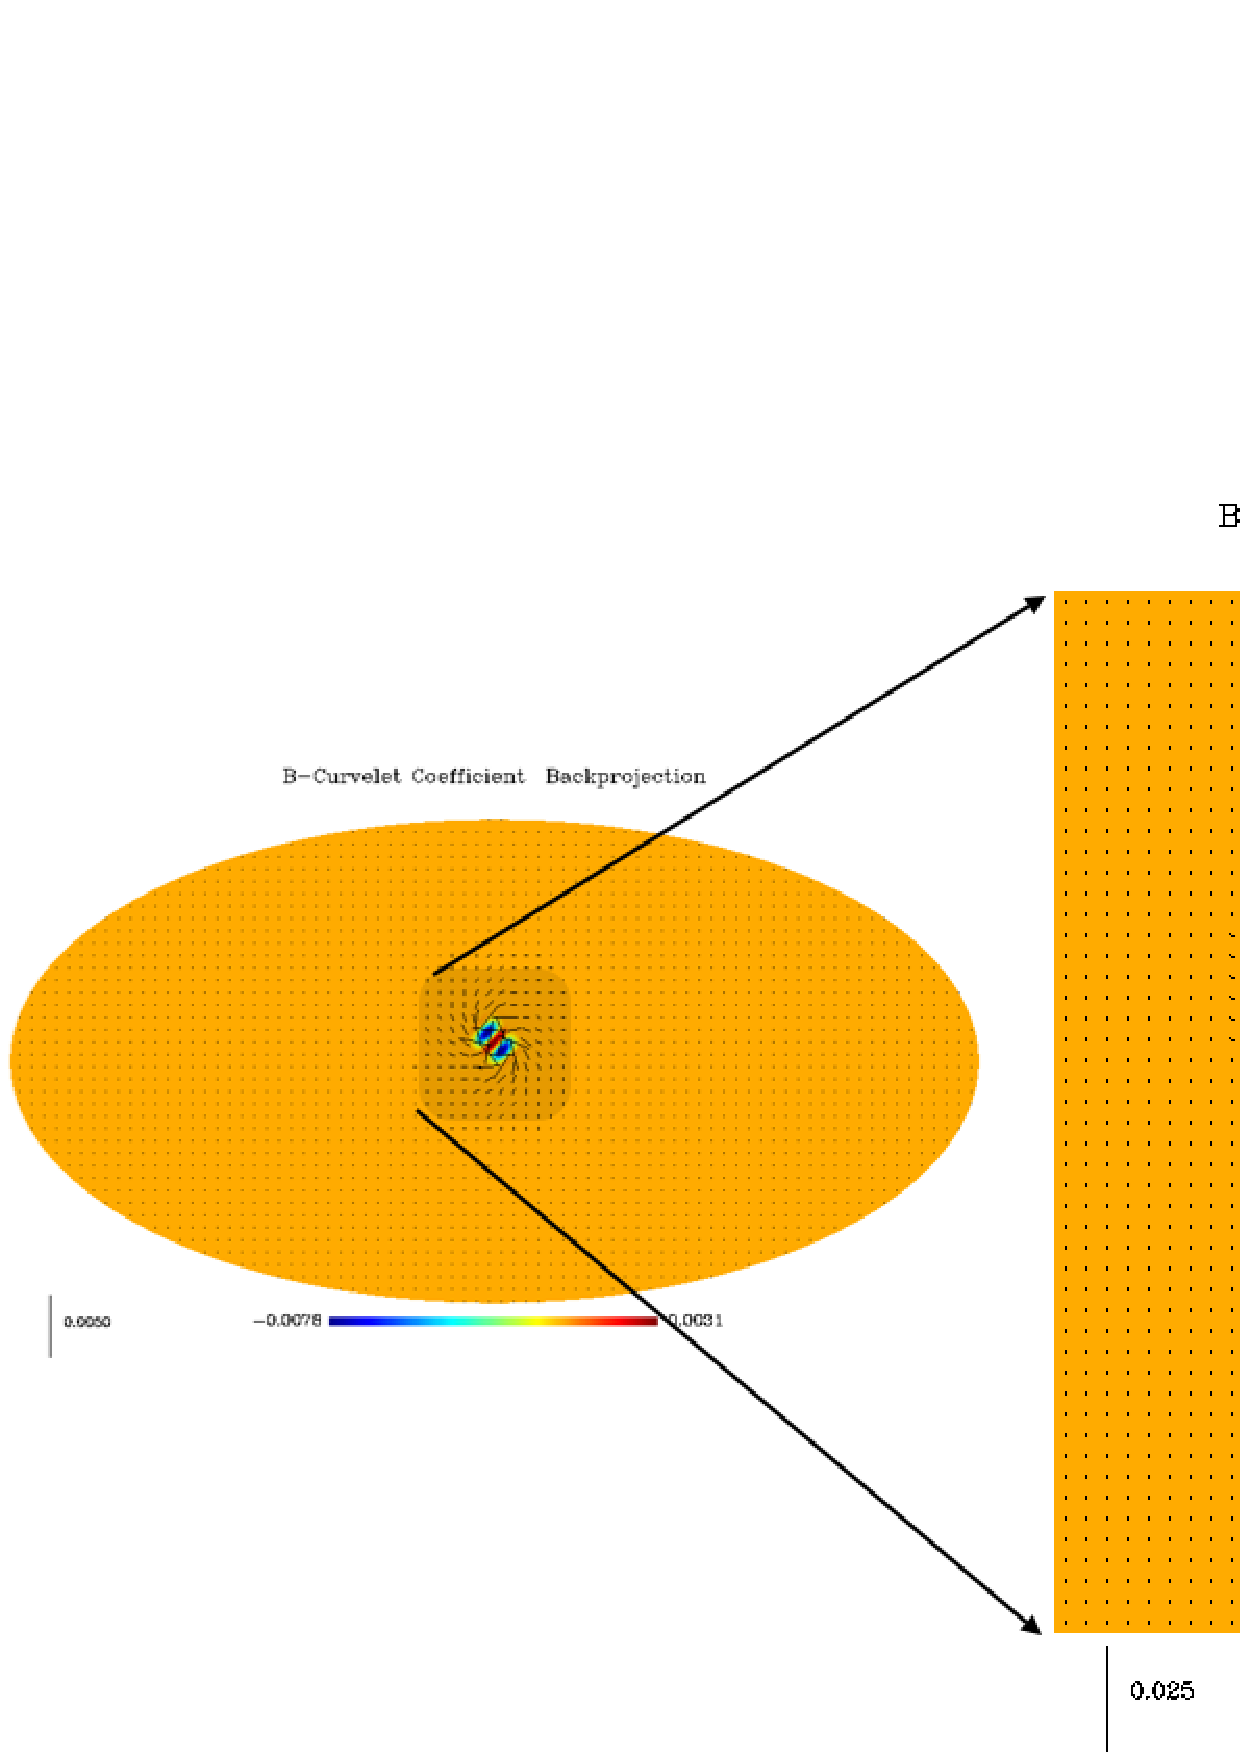
\includegraphics[width=12cm]{fig_bcur_back.pdf}
 }
 }
 }
\caption{B-curvelet coefficient backprojection.}
\label{fig_bcur_back}
\end{figure*}
Similarly to the EB-wavelet constructions, we can easily construct an EB-curvelet transform by first computing the E and B components using 
the spin $\pm 2$ spherical harmonics transform, and then applying a curvelet transform on the sphere separately on each of these two components.
Fig.~\ref{fig_ecur_back} shows the backprojection of an E-curvelet coefficient and Fig.~\ref{fig_bcur_back} shows the backprojectionof a B-curvelet coefficient.

%---------------------------------------------------------------------------------------------------------------------------------------
